\documentclass[a4paper, oneside, openright]{documentationTemplate}

% package to be able to use special characters
\usepackage[latin1]{inputenc}

% Sophisticated math package
\usepackage{amsmath}
\newcommand{\unit}[1]{\ensuremath{\, \mathrm{#1}}}

% Special symbols
\usepackage{amssymb}

% nicely render theorems and proofs
\usepackage[standard,thmmarks,amsmath]{ntheorem}

\usepackage{graphicx}
\usepackage{rotating}

% package to format pseudo-code. Check the package documentation.
\usepackage{algorithmic}
\usepackage{algorithm}
\usepackage{listings}

\usepackage{rotating}

% Provides \xspace command that evaluates to a space if the next character in the source is a blank and
% no space if next character is no blank. Useful in command definitions.
\usepackage{xspace}

% Provides a more flexible tabular environment
\usepackage{tabularx}

% Enables the use of the H location specifier for float environments that puts the float exactly where it is located in the source.
\usepackage{float}

% Enables the use of colours
\usepackage{color}
\usepackage{xcolor}

\definecolor{darkblue}{rgb}{0,0,.5}
\definecolor{Brown}{cmyk}{0,0.81,1,0.60}
\definecolor{OliveGreen}{cmyk}{0.64,0,0.95,0.40}
\definecolor{CadetBlue}{cmyk}{0.62,0.57,0.23,0}
\definecolor{lightlightgray}{gray}{0.9}
\definecolor{lightgreen}{rgb}{0.67, 1, 0.32}


% Enables clickable links in the PDF and additional PDF specific configuration options.
\usepackage[
            colorlinks=true,
            linkcolor=darkblue, urlcolor=darkblue, citecolor=darkblue,
            raiselinks=true,
            bookmarks=true,
            bookmarksopenlevel=1,
            bookmarksopen=true,
            bookmarksnumbered=true,
            hyperindex=true,
            plainpages=false,
            pdfpagelabels=true,
            pdfstartview=FitH,
            pdfstartpage=1,
            pdfpagelayout=OneColumn
            ]{hyperref}

% Enables references to description names
\usepackage{nameref}
\makeatletter
\let\orgdescriptionlabel\descriptionlabel
\renewcommand*{\descriptionlabel}[1]{%
  \let\orglabel\label
  \let\label\@gobble
  \phantomsection
  \edef\@currentlabel{#1}%
  %\edef\@currentlabelname{#1}%
  \let\label\orglabel
  \orgdescriptionlabel{#1}%
}
\makeatother

\usepackage{footnote}
\usepackage{pdfpages}

% Load own command definitions, a few helpful ones are already defined there.

% This alters the numbering of theorems and lemmas.
\theoremsymbol{\ensuremath{\scriptstyle \Diamond}}
\renewtheorem{theorem}{Theorem}[chapter]
\renewtheorem{lemma}[theorem]{Lemma}
\renewtheorem{corollary}[theorem]{Corollary}
\renewtheorem{definition}[theorem]{Definition}

% This creates a two new theorem-like environments
\theoremsymbol{}
\newtheorem{notation}[theorem]{Notation}
\theorembodyfont{}
\newtheorem*{problem}{Problem}

% This changes the comment style of the "algorithmic" pseudocode package
\renewcommand\algorithmiccomment[1]{\hfill \small \(\triangleright\) #1}

% This creates four commands to leave annotations in your document
\newcommand{\TODO}[1]{\noindent {{\color{red}\fbox{\sffamily \bfseries TODO}} \sffamily #1}}
\newcommand{\FIXME}[1]{\noindent {{\color{green}\fbox{\sffamily \bfseries FIXME}} \sffamily #1}}
\newcommand{\CONSIDER}[1]{\noindent {{\color{blue}\fbox{\sffamily \bfseries CONSIDER}} \sffamily #1}}
\newcommand{\RW}[1]{\noindent \color{blue}#1}
\newcommand{\clear}{\newpage{\pagestyle{empty}\cleardoublepage}}

\newcommand{\footnoteremember}[2]{
\footnote{#2}
\newcounter{#1}
\setcounter{#1}{\value{footnote}}
}
\newcommand{\footnoterecall}[1]{
\footnotemark[\value{#1}]
}

% ---------------- highlight inside listings ------------------------------------
\usepackage{etex}
\usepackage{atbegshi,ifthen,tikz}

\tikzstyle{highlighterGreen} = [
  lightgreen,
  line width = \baselineskip,
]

\tikzstyle{highlighterYellow} = [
  yellow,
  line width = \baselineskip,
]

% % implementation Green Highlighter
% \newcounter{highlightGreen}[page]
% \newcommand{\tikzhighlightanchorGreen}[1]{\ensuremath{\vcenter{\hbox{\tikz[remember picture, overlay]{\coordinate (#1 highlightGreen \arabic{highlightGreen});}}}}}
% \newcommand{\bHighlightGreen}[0]{\stepcounter{highlightGreen}\tikzhighlightanchorGreen{begin}}
% \newcommand{\eHighlightGreen}[0]{\tikzhighlightanchorGreen{end}}
% \AtBeginShipout{\AtBeginShipoutUpperLeft{\ifthenelse{\value{highlightGreen} > 0}{\tikz[remember picture, overlay]{\foreach \stroke in {1,...,\arabic{highlightGreen}} \draw[highlighterGreen] (begin highlightGreen \stroke) -- (end highlightGreen \stroke);}}{}}}
%
% % implementation Yellow Highlighter
% \newcounter{highlightYellow}[page]
% \newcommand{\tikzhighlightanchorYellow}[1]{\ensuremath{\vcenter{\hbox{\tikz[remember picture, overlay]{\coordinate (#1 highlightYellow \arabic{highlightYellow});}}}}}
% \newcommand{\bHighlightYellow}[0]{\stepcounter{highlightYellow}\tikzhighlightanchorYellow{begin}}
% \newcommand{\eHighlightYellow}[0]{\tikzhighlightanchorYellow{end}}
% \AtBeginShipout{\AtBeginShipoutUpperLeft{\ifthenelse{\value{highlightYellow} > 0}{\tikz[remember picture, overlay]{\foreach \stroke in {1,...,\arabic{highlightYellow}} \draw[highlighterYellow] (begin highlightYellow \stroke) -- (end highlightYellow \stroke);}}{}}}

%new implementation
\usepackage{highlighter}
\renewcommand{\thepage}{\roman{page}}

% ---------------- end highlight inside listings -------------------------------

%%%%%%%%%%%%%%%%%%%%%%%%%%%%%%%%%%%%%%%%%%%%%%%%%%%%%%%%%%%%%%%%%%%%%%%%%%%%%%%%%%%%%%%%%%%%%%%%%
% DOCUMENT METADATA

\thesistype{Documentation}
\title{Hybrid Fortran v0.97}

\author{Michel M\"uller}
\email{michel@typhooncomputing.com}
\institute{Tokyo Institute of Technology, GSIC \\[2pt]
Typhoon Computing}

% You can put in your own logo here "\includegraphics{...}" or just comment the command
% \logo{}

% You can comment the following two commands if you don't need them
\keywords{Fortran, Weather Prediction, GPGPU, Hybrid, OpenACC, CUDA, TSUBAME, Fermi, Kepler, Tesla, NVIDIA, Westmere, Xeon, Intel, ASUCA}
% \categories{ACM categories go here.}

\date{\today}

% disable hyphenation for a bunch of words

%%%%%%%%%%%%%%%%%%%%%%%%%%%%%%%%%%%%%%%%%%%%%%%%%%%%%%%%%%%%%%%%%%%%%%%%%%%%%%%%%%%%%%%%%%%%%%%%%

\begin{document}

\lstdefinestyle{codestyle} {
  basicstyle=\footnotesize\ttfamily,                   % Code font, Examples: \footnotesize, \ttfamily
  keywordstyle=\color{OliveGreen},        % Keywords font ('*' = uppercase)
  commentstyle=\color{gray},              % Comments font
  numbers=left,                           % Line nums position
  numberstyle=\tiny,                      % Line-numbers fonts
  stepnumber=1,                           % Step between two line-numbers
  numbersep=5pt,                          % How far are line-numbers from code
  %backgroundcolor=\color{lightlightgray}, % Choose background color
  frame=none,                             % A frame around the code
  tabsize=2,                              % Default tab size
  captionpos=b,                           % Caption-position = bottom
  breaklines=true,                        % Automatic line breaking?
  breakatwhitespace=false,                % Automatic breaks only at whitespace?
  showspaces=false,                       % Dont make spaces visible
  showtabs=false,                         % Column format
  morekeywords={},
}

\lstdefinestyle{fortranStyle}{
  language=[90]Fortran,
  style=codestyle
}

\lstdefinestyle{cStyle}{
  language=C,
  style=codestyle
}

\lstset{
  language=[90]Fortran,
  style=codestyle
}

\lstset{emph={
    @parallelRegion, parallelRegion, @domainDependant, domainDependant, @end
    },emphstyle={\color{darkblue}\bfseries}
}

\hyphenation{fortran openacc asuca}

\frontmatter
\maketitle % do not remove this line

\clear
\tableofcontents

\clear
\listoffigures

\clear
\listoftables

\clear
\mainmatter % do not remove this line

\clear
\chapter{The Hybrid Fortran Framework} \label{cha:framework}
Hybrid Fortran is a directive based extension of the and a code transformation tool within the Fortran language. It is intended for enabling GPGPU acceleration of data parallel programs using a unified codebase. Performance Portability was a major design aspect of this framework - not only should it enable the accelerated target to achieve optimal performance, but the CPU target should keep performing as before the migration. In the backend it automatically creates CUDA Fortran code for GPU and OpenMP Fortran code for CPU, in both cases making use of data parallelism defined by the user through directives. Additionally, a GNU Make build system as well as an automatic test system is provided. Hybrid Fortran has been successfully used for speeding up the Physical Core of Japan's national next generation weather prediction model by a factor of 3.6x on Kepler K20x vs. 6 Core Westmere \textit{while not loosing any CPU performance}.

This chapter will describe the functionality of the \textbf{Hybrid Fortran} framework from a user perspective. Chapter \ref{cha:usage} guides through setup, portation, debugging and testing in a 'howto'-like fashion. Chapter \ref{cha:implementation} will go into implementation details for those who would like to adapt \textbf{Hybrid Fortran} to their own specific usecases.

\section{Design Goals} \label{sec:frameworkGoals}

This section gives an overview over the design goals of the \textbf{Hybrid Fortran} framework.

\begin{enumerate}
 \item \textbf{Hybrid Fortran} is intended to enable performance portable parallel programming for HPC purposes.
 \item \label{h90goals:unifiedCodebase} \textbf{Hybrid Fortran} offers a unified codebase for both CPU and GPU execution.

 \item \label{h90goals:compileTimeDefinedStorageOrder} The storage order is compile time defined since CPU and GPU implementations usually have different ideal storage orders.
 \item \label{h90goals:lowComplexity} The rules for creating the GPU code versions should have a low complexity, such that optimizations performed by the user lead to predictable results.
 \item \label{h90goals:performance} The framework enables GPU performance at the level of hand optimized CUDA Fortran while maintaining CPU performance as close as possible to the original CPU code.
 \item \label{h90goals:flexibleImplementation} The implementation details are abstracted from the rest of the system, such that other parallel programming frameworks can be supported in the future without changes in the user code.
 \item \textbf{Hybrid Fortran} is optimized for two use cases in particular: Stencil access patterns with tight loops and Parallel vector access patterns with outside loops. \textbf{Hybrid Fortran} abstracts domain specifications of arrays such that the migration path from typical Fortran code for these two use cases becomes minimal.
\end{enumerate}

\clearpage
\section{Features} \label{sec:features}
\begin{itemize}
 \item Backends for OpenACC (GPU), CUDA Fortran (GPU) and OpenMP (CPU) parallelizations.

 \item Separate parallel regions for CPU and GPU at multiple points in the callgraph (if needed). This allows high performance for both CPU and GPU implementations.

 \item Compile-time defined storage order with different orders for CPU and GPU - all defined in one handy place, the \verb|storage_order.F90| file. Multiple storage orders are supported through attributes in the Hybrid Fortran directives.

 \item Automatic compile time array reformatting - Hybrid Fortran reformats your data with respect to privatization and storage order at compile time. This means you can leave existing Fortran code as is, only the setup using the two Hybrid Fortran directives is needed.

 \item Temporary automatic arrays, module data and imported scalars within GPU kernels (aka subroutines containing a GPU `@parallelRegion`) - this functionality is provided in addition to CUDA Fortran's device syntax features.

 \item Experimental Support for Pointers.

 \item Separate build directories for the automatically created CPU and GPU codes, showing you the created F90 files. Get a clear view of what happens in the back end without cluttering up your source directories.

 \item Use any x86 Fortran compiler for the CPU code (PGI and Intel Fortran have been tested).

 \item Highly human readable intermediate F90 source files. The callgraph, including subroutine names, remains the same as in the user code you specify. The code in the intermediate source files is auto indented for additional reading comfort.

 \item Macro support for your codebase - a separate preprocessor stage is applied even before the hybrid fortran preprocessor comes in, in order to facilitate the DRY principle.

 \item Automatic creation of your callgraph as a graphviz image, facilitating your code reasoning. Simply type `make graphs` in the command line in your project directory.

 \item Automatic testing together with your builds - after an initial setup you can run validation tests as well as valgrind automatically after every build (or by running `make tests`). As an example, say you'd like the preprocessor to tell you that there is a calculation error in array X at point i=10,j=5,k=3? If you set up everything accordingly, this is pretty much what Hybrid Fortran does for you. This speeds up development in large framework a lot, since automated testing means that you can check your work after each submodule or even kernel.

 \item Automatic 'printf' based device debugging mode. Prints all input arrays, output arrays and temporary arrays at the end of each kernel run at a compile-time specified point in a nicely readable format. This output can then be manually validated against the CPU version (which should already produce correct results at that point). Please note: Since PGI's CUDA Fortran does not yet support real device debugging, Hybrid Fortran cannot support that either at this point. However, since the code runs on CPU as well, the class of bugs that are affected by this restriction is rather small (since computational code can be validated on the CPU first) and the current debug mode has been proven to be sufficient for the time being.

 \item Automatic linking and installing of executables. Simply specify the executable names in the `MakesettingsGeneral` configuration file and use corresponding filenames for the main files (which can be placed anywhere in your source tree). The Hybrid Fortran build system will automatically generate the executables (each in CPU and GPU version) and install them in subdirectories of your test directory. The test directories are persistant, such that you can put your initialization files, validation scripts and performance test scripts there. All this happens simply through running `make; make install` in your project directory.
\end{itemize}

\clearpage
\section{Hybrid Fortran Directives} \label{sec:archDirectives}

The directives introduced with the \textbf{Hybrid Fortran} framework are the only additions that have been made to the Fortran 90 language in order to achieve the objectives stated in sec.~\ref{sec:frameworkGoals}. All other syntax elements in \textbf{Hybrid Fortran} are a strict subset of Fortran 90.

It is necessary to introduce the following denotations before introducing the new directives:

\begin{description}
 \item [A domain] in this context denotes a tuple containing a data dimension and its size. For example, if we have an array \verb|a| declared within the range $(1,\unit{NX})$ and looped over using the iterator \verb|x|, we call this array to be \textbf{domain dependant} in domain \verb|x|. For simplicity, we assume that iterators over the same data dimension and range are always named in a consistant way.
 \item [A parallel region] is a code region that can be executed in parallel over a one or more domains.
\end{description}

The following section lists the two directives and their available options for later reference.

\subsection{Parallel Region Directive} \label{sub:parallelRegionDirective}

Listing \ref{listing:parallelRegion} shows the parallel region directive. This directive is an abstraction of for-loops as well as CUDA kernels that allows the framework to define these structures at compile time. It is only allowed to be inserted in the implementation part of a subroutine.

\begin{lstlisting}[name=parallelRegion, label=listing:parallelRegion, caption={Parallel region directive syntax.}]
@parallelRegion{ATTRIBUTE_NAME1(MEMBER1, MEMBER2, ...), ...}
! code to be executed in parallel !
symbol1, symbol2, ...
@end parallelRegion
\end{lstlisting}

The following attributes are supported for this directive:

\begin{description}
 \item [appliesTo] Specify one or more of the following attribute members in order to set this parallel region to apply to either the CPU code version, the GPU version or both. Omitting this attribute has the same effect as specifying all supported architectures.
  \begin{enumerate}
   \item CPU
   \item GPU
  \end{enumerate}
 \item [domName] (Required) Specify one or more domain names over which the code can be executed in parallel. These domain names are being used as iterator names for the respective loops or CUDA kernels.
 \item [domSize] (Required) Set of the domain dimensions in the same order as their respective domain names specified using the \verb|domName| attribute. It is required that $|domName| = |domSize|$.
 \item [startAt] Set the lower boundary for each domain at which to start computations. Omitting this attribute will set all boundaries to \verb|1|. It is required that $|startAt| = |domName|$.
 \item [endAt] Set the upper boundary for each domain at which to end computations. Omitting this attribute will set all boundaries to \verb|domSize| for each domain. It is required that $|startAt| = |domName|$.
 \item [template] Defines a postfix that is to be applied to different attributes that are loaded using the preprocessor. Currently this only affects CUDA Blocksizes: They are loaded using \verb|CUDA_BLOCKSIZE_X_[Template-Name]| from the preprocessor (\verb|storage_order.F90| is the most handy place to define them). The goal of this attribute is to to be able to hoist hardware dependent attributes outside of the code, so when a new architecture comes along, all you need to do is rewriting the template. This functionality will be extended in future Hybrid Fortran releases. Specify this template name without quotes.
\end{description}

Please note: CUDA Fortran differentiates between different subroutine types \cite[p. 4]{CUDAFortranGuide}. Following its design goal of keeping a low complexity, \textbf{Hybrid Fortran} simply rewrites subroutines definitions to one of the CUDA subroutine types, depending on the subroutine's position relative to the parallel region (determined through metainformation about the entire visible source code). This introduces some restrictions for subroutines calling, containing or being called by GPU parallel regions (see also sec.\ref{sec:frameworkRestriction}). For future reference these restricted subroutines are named in the following way (see figure \ref{figure:subroutineTypes}):
\begin{enumerate}
  \item Subroutines that call one or more subroutines containing a GPU parallel region are called \textquotedblleft wrapper subroutines\textquotedblright.
  \item Subroutines that contain a GPU parallel region are called \textquotedblleft kernel subroutines\textquotedblright.
  \item Subroutines that are called inside a GPU parallel region are called \textquotedblleft inside kernel subroutines\textquotedblright.
  \item All other subroutines are called \textquotedblleft host subroutines\textquotedblright.
\end{enumerate}

\subsection{Domain Dependant Directive} \label{sub:domainDependantDirective}

Listing \ref{listing:domainDependant} shows the \textquotedblleft domain dependant\textquotedblright\ directive. It is used to specify the involved symbols and their domain dependencies. This information then allows the framework to rewrite the symbol accesses and declarations for the GPU and CPU cases (see example in section \ref{sub:directiveExample}). Please note the following for using this directive:
\begin{enumerate}
 \item For symbols the framework only operates on local information available for each subroutine. As an example, whether a symbol has already been copied to the GPU is not being analyzed. For this reason the \verb|present| flag has been introduced (see below).
 \item Domain Dependant Directives need to be specified between the specification and the implementation part of a Fortran 90 subroutine.
\end{enumerate}

\begin{lstlisting}[name=domainDependant, label=listing:domainDependant, caption={Domain dependant directive syntax.}]
@domainDependant{ATTRIBUTE_NAME1(MEMBER1, MEMBER2, ...), ...}
! symbols that share the attributes !
! defined above to be defined here, separated  !
! by commas                                    !
...
@end domainDependant

!Minimal Example:
@domainDependant{domName(x), domSize(NX)}
a, b, c
@end domainDependant
!-> Defines the three arrays a, b, c to be dependant in domain x.
\end{lstlisting}

The following attributes are supported for this directive:

\begin{description}
  \item [domName] Set of all domain names in which the symbol needs to be privatized. This needs to be a superset of the domains that are being declared as the symbol's dimensions in the specification part of the current subroutine (except if the \verb|autoDom| attribute flag is used, see below). More specifically, the domain names specified here must be the set of domains from the specification part plus the parallel domains (as specified using the parallel region directive, see section \ref{sub:parallelRegionDirective}) for which privatization is needed.
% $domName_{Domain Dependant}|_{subroutine level} = domName_{Parallel Region}|_$.
 \item [domSize] Set of the domain dimensions in the same order as their respective domain names specified using the \verb|domName| attribute. It is required that $|domName| = |domSize|$.
 \item [accPP \label{descr:accPP}] Preprocessor macro name that takes $|domSize|$ arguments and outputs them comma separated in the current storage order for symbol accesses. This macro must be defined in the file \verb|storage_order.F90| (see section \ref{sub:buildSystem}). In case the \verb|autoDom| attribute is being used, the \verb|accPP| specification is not necessary - \verb|AT|, \verb|AT4|, \verb|AT5| (...) are assumed as defined storage order macro names, depending on the number of array dimensions.
 \item [domPP \label{descr:domPP} ] Preprocessor macro name that takes $|domSize|$ arguments and outputs them comma separated in the current storage order for the symbol declaration. This macro must be defined in the file \verb|storage_order.F90| (see section \ref{sub:buildSystem}). In case the \verb|autoDom| attribute is being used, the \verb|domPP| specification is not necessary - \verb|DOM|, \verb|DOM4|, \verb|DOM5| (...) are assumed as defined storage order macro names, depending on the number of array dimensions. This preprocessor macro is usually identical to the one defined in \verb|accPP|.
 \item [attribute] Attribute flags for these symbols. Currently the following flags are supported:
  \begin{description}
   \item [present] In case this flag is specified, the framework assumes array data to be already present on the device memory for GPU compilation and the data will not be transfered.
   \item [transferHere] In case this flag is specified, all domain dependants with \verb|intent| specified as \verb|in|, \verb|inout| or \verb|out| will be transfered to- and from the device (according to the intent). This flag may not be specified together with the \verb|present| flag (and it should not be necessary, since it has exactly opposite effects).
   \item [autoDom] In case this flag is specified, the framework will use the array dimensions that have been declared using standard Fortran 90 syntax to determine the domains for each symbol. In case the parallel domains are ommitted from the Fortran specification (in order to allow different parallelization for CPU and GPU), they still need to be specified using \verb|domName| and \verb|domSize| for symbols that are to be privatized for each thread. The parallel domains will be inserted before any independent domains picked up through the declaration, depending on the subroutine's position towards the parallel region. In addition, using \verb|autoDom| will by default enable standard \verb|accPP| and \verb|domPP| settings, if not specified otherwise. Using this flag then greatly simplifies the \verb|@domainDependant| specification part, since the directive template (everything between the directive and the corresponding \verb|@end domainDependant| statement) can be reused by symbols of different domains.
   \item [host] In subroutines or modules that are not related to a parallel region in their callgraph, Hybrid Fortran would not know whether a symbol resides on the host or the device. This attribute makes this clear. It is mostly needed in setup code and for module arrays.
  \end{description}
  Please note: In case neither \verb|present| nor \verb|transferHere| is being used, Hybrid Fortran will automatically transfer all domain dependants with \verb|intent| specified as \verb|in|, \verb|inout| or \verb|out| from and to the device according to their intent - \textit{if and only if} the current subroutine is calling a kernel. In other words, the automatic behavior without specifying \verb|present| or \verb|transferHere| in host- or wrapper subroutines will only work if the domain dependants are only used within one wrapper subroutine. For real world callgraphs it is therefore usually necessary to use \verb|present| and \verb|transferHere| attributes in all host- and wrapper subroutines.
\end{description}

An important special case are scalar parameters: In case of a CUDA Fortran implementation, scalars must be passed by value in device functions. The framework must for that reason be aware of scalar symbols in kernel subroutines, such that their specification can be adjusted accordingly. For simplicity reasons, the \verb|@domainDependant| directive has been reused for scalars and can be used in the following way:

\begin{lstlisting}[name=domainDependantScalar, label=listing:domainDependantScalar, caption={Domain dependant directive syntax for scalars.}]
@domainDependant{}
scalar1, scalar2, ...
@end domainDependant
\end{lstlisting}

In \textbf{Hybrid Fortran} terms then, a scalar is a domain dependant without domains. You can however use \verb|attribute(autoDom)| as well here. As a general best practice, you will have two domain dependant directives: One listing the symbols and arrays privatized in the parallel domains and one listing the non privatized symbols and arrays (i.e. they are not variant over these domains).

\subsection{Backend Implementations} \label{sub:backendImplementation}

 Now that the directives have been introduced, you might wonder what exactly Hybrid Fortran is doing with all this. Essentially, the code transformation framework consists of three parts:

 \begin{enumerate}
  \item Parser (Your Hybrid Fortran code including directives).
  \item Callgraph Analysis (Based on the Parser, produces a callgraph coloured by the subroutines' position relative to the parallel regions for CPU and GPU case).
  \item Backend Implementation (For each relevant code point, the Parser calls implementation hooks for the transformation).
 \end{enumerate}
 
 This separation of concerns allows different implementations to be passed in and used, thus enabling portability to different hardware platforms as well as flexibility during development and testing. The implementation class can be chosen using the \verb|MakesettingsGeneral| file in your project's config folder (see also sec. \ref{sub:userDefined}). Table \ref{table:backendImplementationComparison} gives you an overview over the capabilities of each implementation. Adding your own implementation class is as easy as implementing the class in the file \verb|hf_processor/FortranImplementation.py|, using any of the provided classes as a base class and specifying your class name in \verb|MakesettingsGeneral|. For a more detailed look at how to do this, please see also sec. \ref{sub:switchImplementation}.

\tabcolsep=0.11cm
\begin{sidewaystable}[htpb]
        \centering
        \footnotesize
        \begin{tabular}{lllllll}
                Capability/ & \verb|Fortran*| & \verb|OpenMPFortran*| & \verb|PGIOpenACC*| & \verb|CUDAFortran*| & \verb|DebugCUDAFortran*| & \verb|DebugEmulated-| \\
                Class name & & & & & & \verb|CUDAFortran*| \\
                (*='Implementation') & & & & & & \\
                \\
                \hline \hline
                Tested target platforms & Intel x86 & Intel x86 & Nvidia Kepler & Nvidia Kepler & Nvidia Kepler & CUDA emulation mode \\
                \hline
                Tested compilers & Intel, PGI & Intel, PGI & PGI & PGI & PGI & PGI \\
                \hline
                Goal & Basic & OpenMP & OpenACC & CUDA Fortran & Debugging & Debugging \\
                & sequential & CPU & GPU & GPU & CUDA Fortran by & in device \\
                & implementation & Parallelization & Parallelization  & Parallelization & printing one & emulated mode \\
                & & & & & data point for & (allowing \verb|write| \\
                & & & & & each array after & statements within \\
                & & & & & each kernel returns & kernels) \\
                \hline
                Parallel regions & Loops & Loops w/ & Loops w/ & CUDA kernels & CUDA kernels & CUDA kernels \\
                implementation & & OpenMP & OpenACC & & & \\
                & & directives & directives & & & \\
                \hline
                Base class & \verb|object| & \verb|Fortran*| & \verb|Fortran*| & \verb|Fortran*| & \verb|CUDAFortran*| & \verb|DebugCUDAFortran*| \\
                \hline
                Allows multiple & Yes & Yes & Yes & No & No & No \\
                parallel regions & & & & & & \\
                per subroutine & & & & & & \\                
                \hline \hline            
        \end{tabular}
        \caption{Backend Implementations in Hybrid Fortran}
        \label{table:backendImplementationComparison}
\end{sidewaystable}

\subsection{Example} \label{sub:directiveExample}

Let's look at the following example module that performs matrix element addition as well as multiplication. Please note, that the storage order inefficiencies are disregarded in the lst. \ref{listing:exampleCPU}. Also, please note that there are many more examples provided in soure form on \url{http://github.com/muellermichel/Hybrid-Fortran/blog/master/examples/Overview.md}.

\begin{lstlisting}[name=exampleCPU, label=listing:exampleCPU, caption={CPU version of matrix element module}]
module example
contains
subroutine wrapper(a, b, c)
    real, intent(in), dimension(NX, NY, NZ) :: a, b
    real, intent(out), dimension(NX, NY, NZ) :: c
    integer(4) :: x, y
    do y=1,NY
      do x=1,NX
        call add(a(x,y,:), b(x,y,:), c(x,y,:))
        call mult(a(x,y,:), b(x,y,:), c(x,y,:))
      end do
    end do
end subroutine

subroutine add(a, b, c)
    real, intent(in), dimension(NZ) :: a, b, c
    integer :: z
    do z=1,NZ
        c(z) = a(z) + b(z)
    end do
end subroutine

subroutine mult(a, b, d)
    real, intent(in) :: a(NZ), b(NZ)
    real, intent(out) :: d(NZ)
    integer :: z

    do z=1,NZ
      d(z) = a(z) * b(z)
    end do
end subroutine
end module example
\end{lstlisting}

Porting this to the GPU, one might want to move the loops over the \verb|x| and \verb|y| domains to the \verb|add| and \verb|mult| subroutines, in order to eliminate the need for inlining and optimize for register usage. The following listing shows how this is done in \textbf{Hybrid Fortran}. Figure \ref{figure:callgraph} in chap.~\ref{cha:implementation} shows the (programmatically created) callgraph of this module.

\begin{lstlisting}[name=example, label=listing:example, caption={example of a Hybrid Fortran subroutine with a parallel region}]
module example contains
subroutine wrapper(a, b, c, d)
  real, dimension(NZ), intent(in) :: a, b
  real, dimension(NZ), intent(out) :: c, d
  @domainDependant{domName(x,y), domSize(NX,NY), attribute(autoDom)}
  a, b, c
  @end domainDependant
  @parallelRegion{appliesTo(CPU), domName(x,y), domSize(NX, NY)}
  call add(a, b, c)
  call mult(a, b, d)
  @end parallelRegion
end subroutine

subroutine add(a, b, c)
  real, dimension(NZ), intent(in) :: a, b
  real, dimension(NZ), intent(out) :: c
  integer :: z
  @domainDependant{domName(x,y), domSize(NX,NY), attribute(autoDom)}
  a, b, c
  @end domainDependant
  @parallelRegion{appliesTo(GPU), domName(x,y), domSize(NX, NY)}
  do z=1,NZ
      c(z) = a(z) + b(z)
  end do
  @end parallelRegion
end subroutine

subroutine mult(a, b, d)
    real, dimension(NZ), intent(in) :: a, b
    real, dimension(NZ), intent(out) :: d
    integer :: z

    @domainDependant{domName(x,y), domSize(NX,NY), attribute(autoDom)}
    a, b, d
    @end domainDependant

    @parallelRegion{appliesTo(GPU), domName(x,y), domSize(NX, NY)}
    do z=1,NZ
      d(z) = a(z) * b(z)
    end do
    @end parallelRegion
end subroutine
end module example
\end{lstlisting}

This will be rewritten by the \textbf{Hybrid Fortran} framework into two versions. The CPU version will be look like the original (but with an optimized storage order and added OpenMP directives for the parallelization) while the GPU version, using the CUDA Fortran backend implementation, is shown below. Please note, that
\begin{enumerate}
 \item the two implementations loop over the \verb|xy| domains at different points, according to the \verb|appliedTo| attribute defined in the \verb|@parallelRegion| directives. See figure \ref{figure:callgraph} in cha.~\ref{cha:implementation} in order to get an overview.
 \item the declarations and accessors for the arrays \verb|a|, \verb|b|, \verb|c| and \verb|d| did not need to be changed in the \verb|add| and \verb|mult| subroutines.
\end{enumerate}

\begin{lstlisting}[name=exampleGPU, label=listing:exampleGPU, caption={GPU version of the hybrid code shown above}]
module example
contains
  subroutine wrapper(a, b, c, d)
    use cudafor
    real, intent(in) :: a(DOM(NX, NY, NZ)), b(DOM(NX, NY, NZ))
    real ,device :: a_d(DOM(NX, NY, NZ))
    real ,device :: b_d(DOM(NX, NY, NZ))
    real, intent(out) :: c(DOM(NX, NY, NZ)), d(DOM(NX, NY, NZ))
    real ,device :: c_d(DOM(NX, NY, NZ))
    real ,device :: d_d(DOM(NX, NY, NZ))

    type(dim3) :: cugrid, cublock
    integer(4) :: cuerror
    a_d(:,:,:) = a(:,:,:)
    c_d(:,:,:) = 0
    b_d(:,:,:) = b(:,:,:)
    d_d(:,:,:) = 0

    cugrid = dim3(NX / CUDA_BLOCKSIZE_X, NY / CUDA_BLOCKSIZE_Y, 1)
    cublock = dim3(CUDA_BLOCKSIZE_X, CUDA_BLOCKSIZE_Y, 1)
    call add <<< cugrid, cublock >>>(a_d(AT(:,:,:)), b_d(AT(:,:,:)), c_d(AT(:,:,:)))
    ! **** error handling left away to improve readability *** !

    cugrid = dim3(NX / CUDA_BLOCKSIZE_X, NY / CUDA_BLOCKSIZE_Y, 1)
    cublock = dim3(CUDA_BLOCKSIZE_X, CUDA_BLOCKSIZE_Y, 1)
    call mult <<< cugrid, cublock >>>(a_d(AT(:,:,:)), b_d(AT(:,:,:)), d_d(AT(:,:,:)))
    ! **** error handling left away to improve readability *** !

    c(:,:,:) = c_d(:,:,:)
    d(:,:,:) = d_d(:,:,:)
  end subroutine

  attributes(global)   subroutine add(a, b, c)
    use cudafor
    real, intent(in) ,device :: a(DOM(NX, NY, NZ)), b(DOM(NX, NY, NZ))
    real, intent(out) ,device :: c(DOM(NX, NY, NZ))
    integer :: z
    integer(4) :: x, y

    x = (blockidx%x - 1) * blockDim%x + threadidx%x
    y = (blockidx%y - 1) * blockDim%y + threadidx%y
    do z=1,NZ
      c(AT(x,y,z)) = a(AT(x,y,z)) + b(AT(x,y,z))
    end do
  end subroutine

  attributes(global) subroutine mult(a, b, d)
    use cudafor
    real, intent(in) ,device :: a(DOM(NX, NY, NZ)), b(DOM(NX, NY, NZ))
    real, intent(out) ,device :: d(DOM(NX, NY, NZ))
    integer :: z
    integer(4) :: x, y

    x = (blockidx%x - 1) * blockDim%x + threadidx%x
    y = (blockidx%y - 1) * blockDim%y + threadidx%y
    do z=1,NZ
      d(AT(x,y,z)) = a(AT(x,y,z)) * b(AT(x,y,z))
    end do
  end subroutine
end module example
\end{lstlisting}

\clearpage
\section{Restrictions} \label{sec:frameworkRestriction}

The following restrictions will need to be applied to standard Fortran 90 syntax in order to make it compatible with the \textbf{Hybrid Fortran} framework in its current state. For the most part these restrictions are necessary in order to ensure CUDA Fortran compatibility. Other restrictions have been introduced in order to reduce the program complexity while still maintaining suitability for common physical packages.

\begin{figure}[htpb]
	\centering
	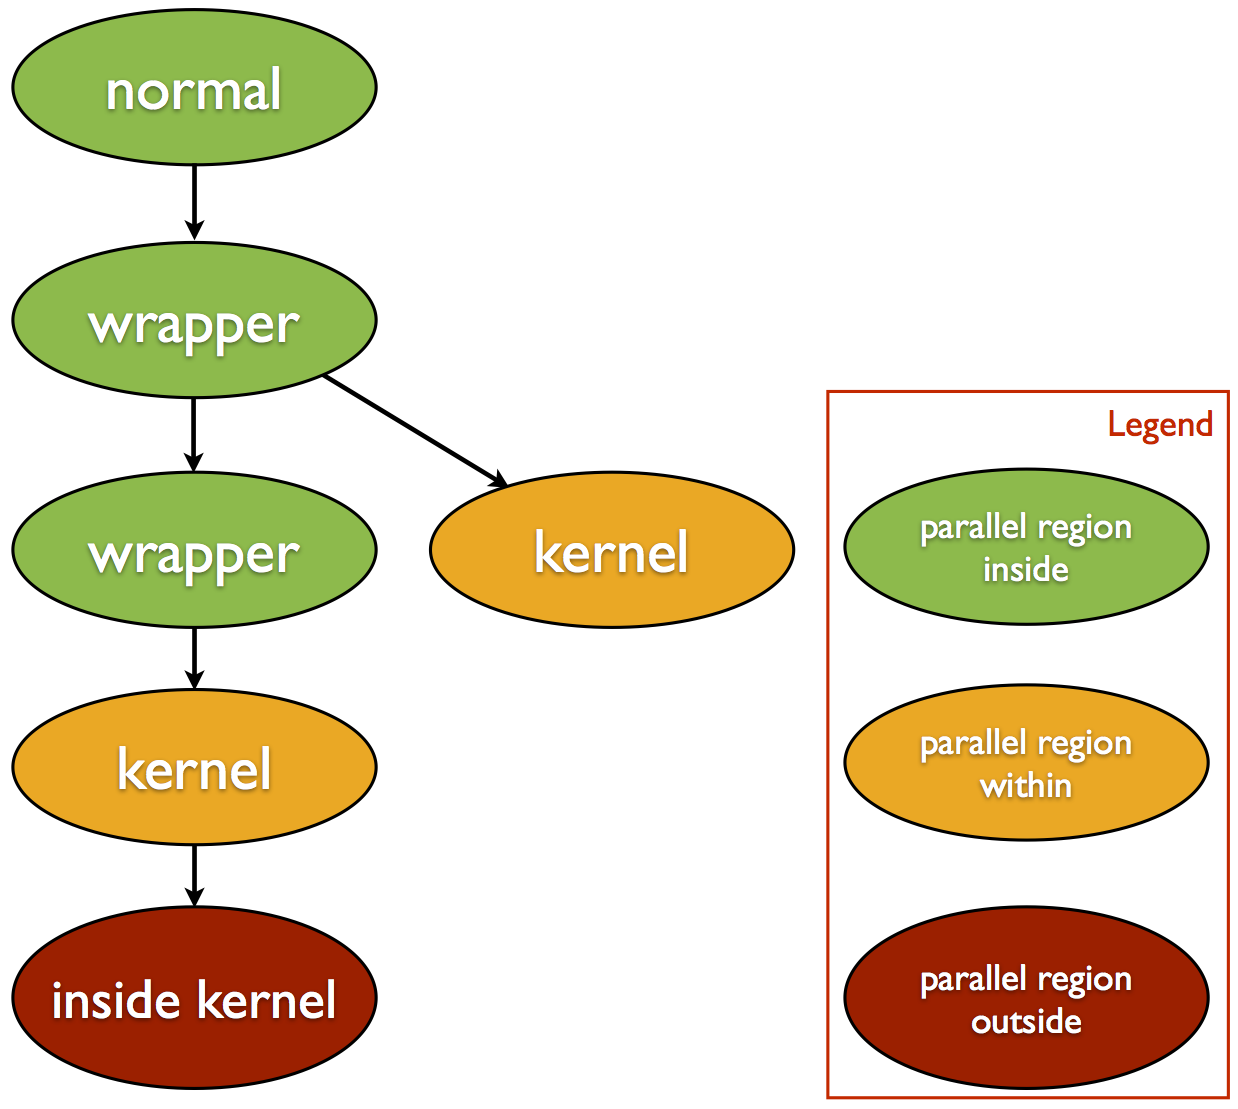
\includegraphics[width=7.5cm]{figures/subroutineTypes.png}
	\caption[Hybrid Fortran Subroutine Types]{Callgraph showing subroutine types with restrictions for GPU compilation.}
	\label{figure:subroutineTypes}
\end{figure}

\begin{enumerate}
 \item Hybrid Fortran has only been tested using free form Fortran 90 and Fortran 2003 syntax.
 \item Your free form files will need the f90 or F90 file endings for the Hybrid Fortran build system to pick them up (this is also recommended by Intel if you want to use their compiler).
 \item Support for pointers in kernel callers is still experimental. See the \verb|diffusion3D| example for an example code on how to use pointers together with Hybrid Fortran. All pointers that are to touch the device need a specified intent and their domain / dimension setup needs to be specified within a domainDependant directive.
 \item Hybrid Fortran currently supports data parallel programming for multicore CPU and GPU. In order to use reduce functions, it is recommended to use BLAS/CUBLAS (see poisson2d solver example).
 \item Currently no line continuations are supported for the attribute definitions of directives.
 \item Because of OpenACC / CUDA Fortran restrictions, kernel- and inside kernel subroutines may not
  \begin{enumerate}
   \item contain symbols declared with the \verb|DATA| or \verb|SAVE| attribute.
   \item contain multiple parallel regions.
   \item be recursive.
   \item call other kernel subroutines.
   \item contain the \verb|recursive|, \verb|pure| and \verb|elemental| keywords.
   \item contain inline array initialisations. Static data initialisations are ideally being done outside the parallel loop, typically in \verb|init| subroutines for each module that are always executed on the CPU. \textbf{Hybrid Fortran} directives are not needed for code parts that are in no case to be executed on the GPU, however the compile time storage order needs to be be respected by using the same storage order macros as specified in the \ref{descr:domPP} and \ref{descr:accPP} attributes for the involved arrays. Alternatively you can specify \verb|@domainDependant| directives in these code parts, so HF will take over the storage order handling.
  \end{enumerate}
 \item Inside kernel subroutines called by kernel subroutines must reside in the same Fortran module as their caller.
 \item All symbols that are declared as domain dependant using \verb|@domainDependant| directives must be of \verb|integer|, \verb|real|, \verb|character| or \verb|logical| type (however any byte length within the Fortran 90/2003 specification is allowed). Hybrid Fortran doesn't currently have support for derived types containing data arrays that need to be copied onto the device. You can use derived types in host-only code however.
 \item Arrays that are declared as domain dependant using \verb|@domainDependant| directives may not appear in declaration lines with mixed domain dependance. Example:
 \begin{lstlisting}[name=exampleMixedOK, label=listing:exampleMixedOK, caption={This is ok.}]
 ..
 real(8), dimension(nz) :: a, b
 real(8), dimension(nz) :: c
 ..
 @domainDependant {domName(x), domSize(nx)}
 a, b
 @end domainDependant

 @domainDependant {domName(y), domSize(ny)}
 c
 @end domainDependant
 ..
 \end{lstlisting}

 \begin{lstlisting}[name=exampleMixedNotOK, label=listing:exampleMixedNotOK, caption={This is not ok.}]
 ..
 real(8) dimension(nz) :: a, b, c
 ..
 @domainDependant {domName(x), domSize(nx)}
 a, b
 @end domainDependant

 @domainDependant {domName(y), domSize(ny)}
 c
 @end domainDependant
 ..
 \end{lstlisting}
 \item The regular Fortran 90 declarations of any symbols declared as domain dependant may not contain line continuations.
 \item Use statements in kernel- and inside kernel subroutines may not contain line continuations.
 \item All source files (h90\footnote{h90 is the file extension used for Hybrid Fortran source files.}, H90\footnote{H90 is the file extension used for Hybrid Fortran source files that contain same-file macro expansions.}, f90, F90) need to have distinctive filenames since they will be copied into flat source directories by the build system.
 \item Subroutines in h90 and H90 files need distinctive names for the entire source tree.
 \item Only subroutines are supported together with \textbf{Hybrid Fortran} directives, e.g. functions are not supported.
 \item Preprocessor directives that affect the Hybrid Fortran preprocessing (such as code macros) must be expandable from definitions within the same H90 file. Use the H90 file suffix (instead of h90) in case you want to use macros in your code.
 \item If you use local module scalars inside a kernel subroutine, the wrapper subroutine must reside in the same module.
 \item Module scalars, when used in a kernel subroutine, will loose their constant characteristic on GPU. They therefore can't be used where a constant is required, such as in a \verb|case| statement. (They do work as a dimension specifier for automatic arrays however.)
 \item I/O statements such as \verb|read| or \verb|write| and \verb|STOP| statements are not possible inside GPU parallel regions, except for emulated mode.
\end{enumerate}

In general, since
\begin{enumerate}
  \item GPU execution currently requires subroutine calls to be inlined and
  \item the number of registers per GPU Streaming Multiprocessor is limited
\end{enumerate}
it is best to split deep callgraphs and large computations into multiple smaller kernels (i.e. \verb|@parallelDomain{ appliedTo(GPU), ..}|).

\clearpage
\section{Device Data Handling} \label{sec:deviceDataHandling}
The goal of device data handling is to hide and abstract code that is only necessary for the CUDA execution path. \textbf{Hybrid Fortran} works similarly to OpenACC in that respect. For all non-scalars that are marked as domain dependant using the \verb|@domainDependant| directive, the following rules apply with respect to device data in case of GPU compilation:
\begin{enumerate}
  \item If the current subroutine contains calls to kernel subroutines and the domain dependant symbol is declared using the \verb|intent(in)| or \verb|intent(inout)| statement, a device version of the symbol will be allocated and its content will be copied to that device array at the beginning of the subroutine.
  \item If the current subroutine contains calls to kernel subroutines and the domain dependant symbol is declared using the \verb|intent(out)| or \verb|intent(inout)| statement, a device version of the symbol will be allocated and set to zero and the device array's content will be copied to the original array at the end of the subroutine.
  \item If the domain dependant symbol is local for this subroutine, it will be allocated as a device symbol and its content will be set to zero at the beginning of the subroutine.
  \item In case the domain dependant directive contains an \verb|attribute(present)| statement, no data will be copied and the original symbol will be declared as a device symbol.
  \item In case the domain dependant directive contains an \verb|attribute(transferHere)| statement, the data will always copied over to the device, following the specified intents (as in (1), (2)). 
\end{enumerate}

\subsection{Module Data}
Using the following guidelines, Hybrid Fortran is able to manage your imported module data to be copied to and from the device.
\begin{enumerate}
 \item After the specification part of your module, add \verb|@domainDependant| directives and include all arrays that need to be touched by your parallel regions.
 \item In case your module data arrays are allocatable (which is probably the case if your problem dimensions are runtime defined), you cannot use \verb|attribute(autoDom)|. Instead, use the \verb|domName| and \verb|domSize| attributes to specify the domain setup. You may use runtime defined scalar variables (e.g. \verb|nx|, \verb|i|, ...) within this specification as long as these variables are always defined within the parallel regions that use these arrays. These runtime variables do \textbf{not} need to be imported into the declaring module.
 \item Specify \verb|attribute(host)| for all these arrays in the module specification.
 \item In the module data consuming kernel subroutine, simply import the data with \verb|use| statements (please note that Hybrid Fortran cannot parse multiline \verb|use| statements at this point). And specify them also inside the corresponding \verb|domainDependant| directive. You may use \verb|attribute(autoDom)| there, since Hybrid Fortran will use the domain information that you provide in the module specification. The data handling at this point follows the same rules as locally declared arrays (see above) - so make sure that you use \verb|attribute(present)| and \verb|attribute(transferHere)| if you have multiple kernel subroutines that touch the same data.
\end{enumerate}

\clearpage
\section{Feature Comparison between Hybrid Fortran and OpenACC} \label{sec:featureComparisonFrameworks}

The following table gives an overview over the differences between OpenACC and the \textbf{Hybrid Fortran} framework.

\begin{table}[htpb]
	\centering
	\footnotesize
	\begin{tabular}{l|c|c|l}
		Feature & OpenACC & Hybrid & Comments \\
		& & Fortran 90 & \\
		\hline \hline
		Enables close to fully optimized  & & \checkmark & CUDA Fortran implementation \\
		Fortran code for GPU execution & & & available, which has equal or better \\
		& & & performance than OpenACC in all \\
		& & & cases known to us \\
		\hline
		Enables close to fully & & \checkmark & Storage order abstraction as well \\
		optimized Fortran code & & & as allowing both coarse grained \\
		for CPU execution & & & as well as fine grained parallelization \\
		& & & leads to this result. \\
		\hline
		Automatic device data & \checkmark & \checkmark & \\
		copying & & & \\
		\hline
		Allows adjusted looping & & \checkmark & \\
		patterns for CPU and & & & \\
		GPU execution & & & \\
		\hline
		Allows changing the & & \checkmark & \\
		looping patterns with & & & \\
		minimal adjustments in & & & \\
		user code & & & \\
		\hline
		Handles compile time & & \checkmark & \\
		defined storage order & & & \\
		\hline
		Allows to adapt & & \checkmark & Details, see section \ref{sub:switchImplementation} \\
		for other technologies & & & \\
		without changing the user & & & \\
		code (e.g. switching to & & & \\
		OpenCL) & & & \\
		\hline
		Allows arbitrary access & \checkmark & \checkmark &  \\
		patterns in parallel & & & \\
		domains & & & \\
		& & & \\
		& & & \\
		\hline
		Allows multiple parallel & \checkmark & (\checkmark) & HF: Only OpenACC backend. \\
		regions per subroutine & & & \\
		\hline
		Generated GPU code remains & & \checkmark & OpenACC compiles to CUDA C \\
		easily human & & & (PGI), introduces new \\
		readable & & & functions for device kernels. \\
		& & & Hybrid Fortran can translate to \\
		& & & CUDA Fortran, code remains \\
		& & & easily readable.\\
		\hline
		Allows debugging of & \checkmark & \checkmark & \\
		device data & & & \\
		\hline
		Framework Sourcecode & & \checkmark & \\
		available & & & \\
		\hline
	\end{tabular}
	\caption{Feature Comparison OpenACC vs. Hybrid Fortran}
	\label{table:featureComparisonFrameworks}
\end{table}




\clear
\chapter{Usage of the Hybrid Fortran Framework} \label{cha:usage}

This chapter is intended to give the informations necessary for installing and using the \textbf{Hybrid Fortran} framework.

\section{Framework Dependencies} \label{sec:dependencies}

\textbf{Hybrid Fortran} requires the following software components:

\begin{enumerate}
 \item A compiler for either OpenACC Fortran (Cray or PGI (only PGI tested so far)) or CUDA Fortran (PGI).
 \item An x86 Fortran compiler.
 \item Python v2.6.x, Python v2.7.x or compatible.
 \item GNU Make 3.81.
 \item A POSIX compatible operating system.
 \item (optional) \verb|valgrind| is recommended if you would like to use the test system shipped with this framework (accessible through \verb|make tests|).
 \item (optional) Allinea DDT if you need parallel debugging on the device.
 \item (optional) For the graphical callgraph representation using \verb|make graphs|: ``pydot'' python library\footnote{http://code.google.com/p/pydot/} as well as the ``Graphviz'' program package\footnote{http://www.graphviz.org/Download..php}.
 \item (optional) \verb|NetCDF4-Python| and \verb|numpy| in case you'd like to use Hybrid Fortran's automated testing together with NetCDF Output.
\end{enumerate}

\section{User Defined Components} \label{sub:userDefined}

The following files displayed in figure \ref{figure:hybridCUDAComponentsAndInfoFlow} are defined by the user:

\begin{description}
 \item[h90(H90) Fortran sources] A source directory that contains Hybrid Fortran files (h90/H90 extension). It may also contain files with f90 or F90 extensions. The source directory is by default located at \verb|path-to-project/source/*| (this can be changed in the \verb|path-to-project/config/MakesettingsGeneral| file).
 \item[Makefile] Used to define module dependencies. The Makefile is by default located at \verb|path-to-project/buildtools/Makefile|. Note: All source files are being copied into flat source folders before being compiled - the build system is therefore source directory structure agnostic, i.e. files can be placed into arbitrary subdirectores below the source directory.
  \item[MakesettingsCPU] CPU compiler settings are specified in \verb|MakesettingsCPU|, located at \verb|path-to-project/buildtools/|.
  \item[MakesettingsGPU] GPU compiler settings are specified in \verb|MakesettingsGPU|, located at \verb|path-to-project/buildtools/|.
  \item[MakesettingsGeneral] Common settings, such as executable file names, the choice Hybrid Fortran preprocessor implementation class, or files and folders being excluded from compilation. With the helper comments these settings should be self explanatory.
 \item[storage\_order.F90] This fortran file contains fortran preprocessor statements in order to define the storage order for both CPU and GPU implementation. It can be placed anywhere in the source directory or its subdirectories (see above).
\end{description}

\section{Build Interface} \label{sub:buildInterface}

\begin{description}
 \item[make] builds both cpu and gpu versions of the codebase situated in \linebreak\verb|path-to-project/source/*|.
 \item[make build\_cpu] builds the cpu version of the codebase situated in \verb|path-to-project/source/*|.
 \item[make build\_gpu] builds the gpu version of the codebase situated in \verb|path-to-project/source/*|.
 \item[make install] builds both cpu and gpu versions of the codebase situated in \verb|path-to-project/source/*| and installs the executables into the test folder defined in \verb|path-to-project/buildtools/MakesettingsGeneral|.
 \item[make install\_cpu] Like \verb|make install|, but only for the cpu version.
 \item[make install\_gpu] Like \verb|make install|, but only for the gpu version.
 \item[make clean] Removes the build directories as well as cpu executables from the test folders.
 \item[make clean\_cpu] Like \verb|make clean|, but only for the cpu version.
 \item[make clean\_gpu] Like \verb|make clean|, but only for the gpu version.
 \item[make tests] Executes \verb|make install| and runs the automatic tests (see sec. ~\ref{sec:testSystem}) for all executables.
 \item[make tests\_cpu] Like \verb|make tests|, but only for the cpu version.
 \item[make tests\_gpu] Like \verb|make tests|, but only for the gpu version.
 \item[make TARGETS DEBUG=1] builds TARGETS in debug mode (use any of the targets defined above). Uses the \verb|DebugCUDAFortranImplementation| in case of GPU compilation (by default), which prints predefined data points for every kernel parameter after every kernel execution. See also the flag \verb|DEBUG_MODE| in \verb|MakesettingsGeneral| which allows to use the debug mode by default.
 \item[make TARGETS VERBOSE=1] builds TARGETS with more detailed output.
 \item[make graphs] creates the graphical callgraph representations in the \linebreak\verb|path-to-project/build/callgraphs/| directory.
\end{description}

\section{Test Interface} \label{sec:testSystem}
\textbf{Hybrid Fortran} comes with an automated test system that - once set up - is intended to find all errors in your code, each time a build completes. This includes
\begin{itemize}
 \item Initialization errors (symbols / arrays being read without initializing them first), using \verb|valgrind|.
 \item Memory handling errors (in case you forget to deallocate arrays), using \verb|valgrind|.
 \item Computational errors, using reference data. Currently supported for this validation is output in \verb|NetCDF| format as well as standard Fortran \verb|.DAT| files. For NetCDF, up to five data dimensions per variable are supported, for .DAT files it is up to three dimensions.
\end{itemize}

\subsection{Integration} \label{sub:testIntegration}
If you would like to integrate the provided system, please do the following:
\begin{enumerate}
  \item \label{enum:writeProc} Choose between the following options for your output.
    \begin{enumerate}
      \item Have your program output in NetCDF format. In that case you will need \verb|numpy| as well as \verb|NetCDF-Python| installed as additional dependencies. It is recommended to install these dependencies into a \verb|virtualenv| such that you can use a different compilers for the post processing as for the program itself (you will need NetCDF compiled in both versions). Compiling the entire post processing stack with PGI compilers (all of python, numpy) is not recommended. You can then use the \verb|SOURCE_THIS_BEFORE_TESTING| and \verb|SOURCE_THIS_AFTER_TESTING| options in \verb|MakesettingsGeneral| to specify the activate and deactivate scripts for your virtualenv. In case of NetCDF, the Hybrid Fortran test system will automatically pick up any variable in your output and test it against the reference.
      \item Add calls to the \verb|helper_functions| module procedures \verb|write1DToFile|, \verb|write2DToFile| and \verb|write3DToFile| to your program to be tested in order to write your data to the \verb|.dat| files in the \verb|test\your-executable\out| folder. The \verb|helper_functions| module is part of the Hybrid Fortran libraries and it is always included in Hybrid Fortran builds - in fact it gets copied into your build directories for consistancy reasons. You may choose any filename for the \verb|.dat| files, the \verb|allAccuracy.py| script will find them automatically in the \verb|test\your-executable\out| folder.
    \end{enumerate}
  \item \label{enum:testCompile1} Compile (\verb|make; make install| in project directory) and run your program to make sure the files are being created. Make sure that they actually contain data, for example by checking the file size.
  \item Repeat steps \ref{enum:writeProc}, \ref{enum:testCompile1} in your reference source code in case you go for the .DAT-files option.
  \item Compress the reference data created by your reference program into \linebreak\verb|./test/your-executable/ref.tar.gz|. See also the description of \verb|runTest.sh| in conjunction with the \verb|validation| command below to understand the correct format.
  \item During development of your hybrid codebase, set the flags \verb|TEST_WITH_EVERY_BUILD| and \verb|DEBUG_MODE| to \verb|true| in the file \verb|MakesettingsGeneral|. This ensures that your tests will run with every build of Hybrid Fortran.
\end{enumerate}

\subsection{Interface} \label{sub:testInterface}
The following files are part of the sample test interface provided with \textbf{Hybrid Fortran}. They are located in the framework's binary directory. In order to set up the test system correctly, what's relevant for you is the information provided for the files \verb|runTest.sh| and \verb|runTests.sh|. The other files are described here for completeness and in case you'd like to adapt the system for different use cases.

\begin{description}
 \item [accuracy.py] Compares one NetCDF - or Fortran 90 \verb|.dat| file with a reference file. Endianness, number of bytes per floating point value can be specified for the \verb|.dat| case using command line parameters. See \verb|--help| for usage.
 \item [allAccuracy.sh] Compares all Fortran 90 \verb|.dat| files or NetCDF files according that match a filename pattern. By default, the pattern \verb|./out/*.dat| is used - you can override this by defining \verb|TEST_OUTPUT_FILE_PATTERN| in MakesettingsGeneral.
 \item [runTest.sh] Executes a series of tests for one executable. In order to use this, please \verb|cd| into the executable's test directory first. This script takes three mandatory and three optional command line arguments :
  \begin{enumerate}
   \item The path to the executable as seen from its working directory.
   \item The architecture name for which the tests should be performed (currently either \verb|cpu| or \verb|gpu|).
   \item The postfix of the command line argument specification file. These files with filename \verb|testConfig_[postfix].txt| should be placed in the executable's test directory for this matter. Each line in these text files will be interpreted as follows: \linebreak
   \verb|arg_name1 arg_value1 arg_name2 arg_value2 ...|. All lines need to have the same number of command line arguments specified. The executables to be used with this test system are assumed to have a unix-style command line interface. This can easily be achieved using the \verb|kracken| Fortran module, already provided with Hybrid Fortran (for its documentation, see \cite{Kracken}). As an example, the following command line argument specification file will call the executable once with arguments \verb|-nx 1 -ny 2| and once with \verb|-nx 2 -ny 3|:
\begin{lstlisting}[name=commandLineSpecification, label=listing:commandLineSpecification, caption={A sample command line argument specification file}]
nx 1 ny 2
nx 2 ny 3
\end{lstlisting}. By using different postfixes you can define any number of configuration files that can then be used together with \verb|runTest.sh|. Please note that the following postfixes have a special meaning:
    \begin{description}
     \item [validation] attempts to extract the reference data from the file \verb|ref.tar.gz| (which is to be located inside the executable's test directory) and runs \verb|allAccuracy.sh| with matching reference directories named using the schema \verb|./ref_[arg_name1][arg_value1]_[...]/|. As an example, if you'd like to use the specification file as shown in lst. \ref{listing:commandLineSpecification}, you will need to provide a file \verb|ref.tar.gz| that contains the following reference data directories: \verb|ref_nx1_ny2| and \verb|ref_nx2_ny3|. Use the command \verb|tar -cvzf ref.tar.gz ref_*| to create this file once you have the reference data ready. In order to create
     \item [valgrind] calls valgrind tests with these command line specifications. This should only be used for cpu executables that have been compiled using debug flags (\verb|-g|).
    \end{description}
   \item (optional) The output file pattern for your executable. See also the setting \verb|TEST_OUTPUT_FILE_PATTERN| in \verb|config/MakesettingsGeneral|.
   \item (optional) The path to a script that is to be sourced before running validation tests (see also step \ref{enum:writeProc} in section \ref{sub:testIntegration}).
   \item (optional) The path to a script that is to be sourced after running validation tests.
  \end{enumerate}
 \item [runTests.sh] This script \verb|cd|'s into the test directories and runs \verb|validation| as well as \verb|valgrind| tests (for cpu executables when the debug argument is being passed to this script) for all specified executables. This assumes that you have specified command line argument specification files for those two test cases (see above). \verb|runtests.sh| takes the following arguments:
  \begin{enumerate}
   \item A list of paths to executables.
   \item The mode in which the executables should be run - currently \verb|debug| or \verb|production|.
   \item The architecture name for which the tests should be performed (currently either \verb|cpu| or \verb|gpu|).
   \item (optional) The output file pattern for your executable. See also the setting \verb|TEST_OUTPUT_FILE_PATTERN| in \verb|config/MakesettingsGeneral|.
   \item (optional) The path to a script that is to be sourced before running validation tests (see also step \ref{enum:writeProc} in section \ref{sub:testIntegration}).
   \item (optional) The path to a script that is to be sourced after running validation tests.
  \end{enumerate}
  By setting the \verb|TEST_WITH_EVERY_BUILD| flag to \verb|true| in the file \verb|config/MakesettingsGeneral|, every build will automatically run \verb|runTests.sh| with the executable list used for compilation as well as the correct debug flag.
\end{description}

\section{Getting Started}
\begin{enumerate}
 \item Clone \url{http://github.com/muellermichel/Hybrid-Fortran} to your computer used for development. Make sure your system meets the dependencies specified in section \ref{sec:dependencies}.
 \item Set the environment variable \verb|HF_DIR| to the location under which you have installed Hybrid Fortran.
 \item \verb|cd| into the Hybrid Fortran directory you've now installed on your computer.
 \item Run \verb|make example|. This creates a new project directory named \verb|example|.
 \item Run \verb|cd example|.
 \item Run \verb|make; make install|. If everything worked you should now have a test subdirectory containing the example subdirectory containing two executables, one for CPU and one for GPU execution. Otherwise it is likely that some dependencies are missing, please reconsider section \ref{sec:dependencies}.
 \item Run \verb|./test/example/example_cpu; ./test/example/example_gpu|. This should execute and validate both versions.
 \item Review the example source files located in \verb|./source| and get a feel for the Hybrid Fortran directive syntax. Notice the \verb|storage_order.F90| file which is used as a central point for specifying the data storage orders. Please refer to the documentation for details.
 \item Review the preprocessed source files located in \verb|./build/cpu/source| and \verb|./build/gpu/source|. Notice the OpenMP and CUDA code that has been inserted into the example codebase. These files are important for debugging as well as when you want to do manual performance optimizations (but you should usually never change anything there, since it will get overwritten with the next preprocessor run).
 \item Review the config files located in \verb|./config|. The most important file for integrating your own codebase will be \verb|./config/Makefile|. This file specifies the dependency tree for your source files. Please note that \verb|vpath|'s are not necessary, the Hybrid Fortran build system will find your source files automatically, as long as you use the source directory specified in \verb|./config/MakesettingsGeneral| as the root of your sources (i.e. you may place your sources in an arbitrarily deep subdirectory structure). The \verb|MakesettingsCPU| and \verb|MakesettingsGPU| are used to define the compilers and compiler flags. You may use any CPU compiler, however only \verb|pgf90| is currently supported for CUDA compilation.
 \item Run \verb|make clean; make DEBUG=1; make install| in your example project directory. This replaces the previously compiled executables with debug mode executables.
 \item The CPU version can be debugged with a compatible debugger.
 \item Run \verb|./test/example/example_gpu| and notice how this executable now prints debug information for every input and output at a specific data point after every kernel run. You can change the data point in \verb|storage_order.F90|.
 \item Rename the example project directory to your project name and start integrating your codebase. You can move it to any directory you'd like.
\end{enumerate}

\section{Migration to Hybrid Fortran with CUDA Fortran Backend}

\begin{figure}[hbtp]
  \centering  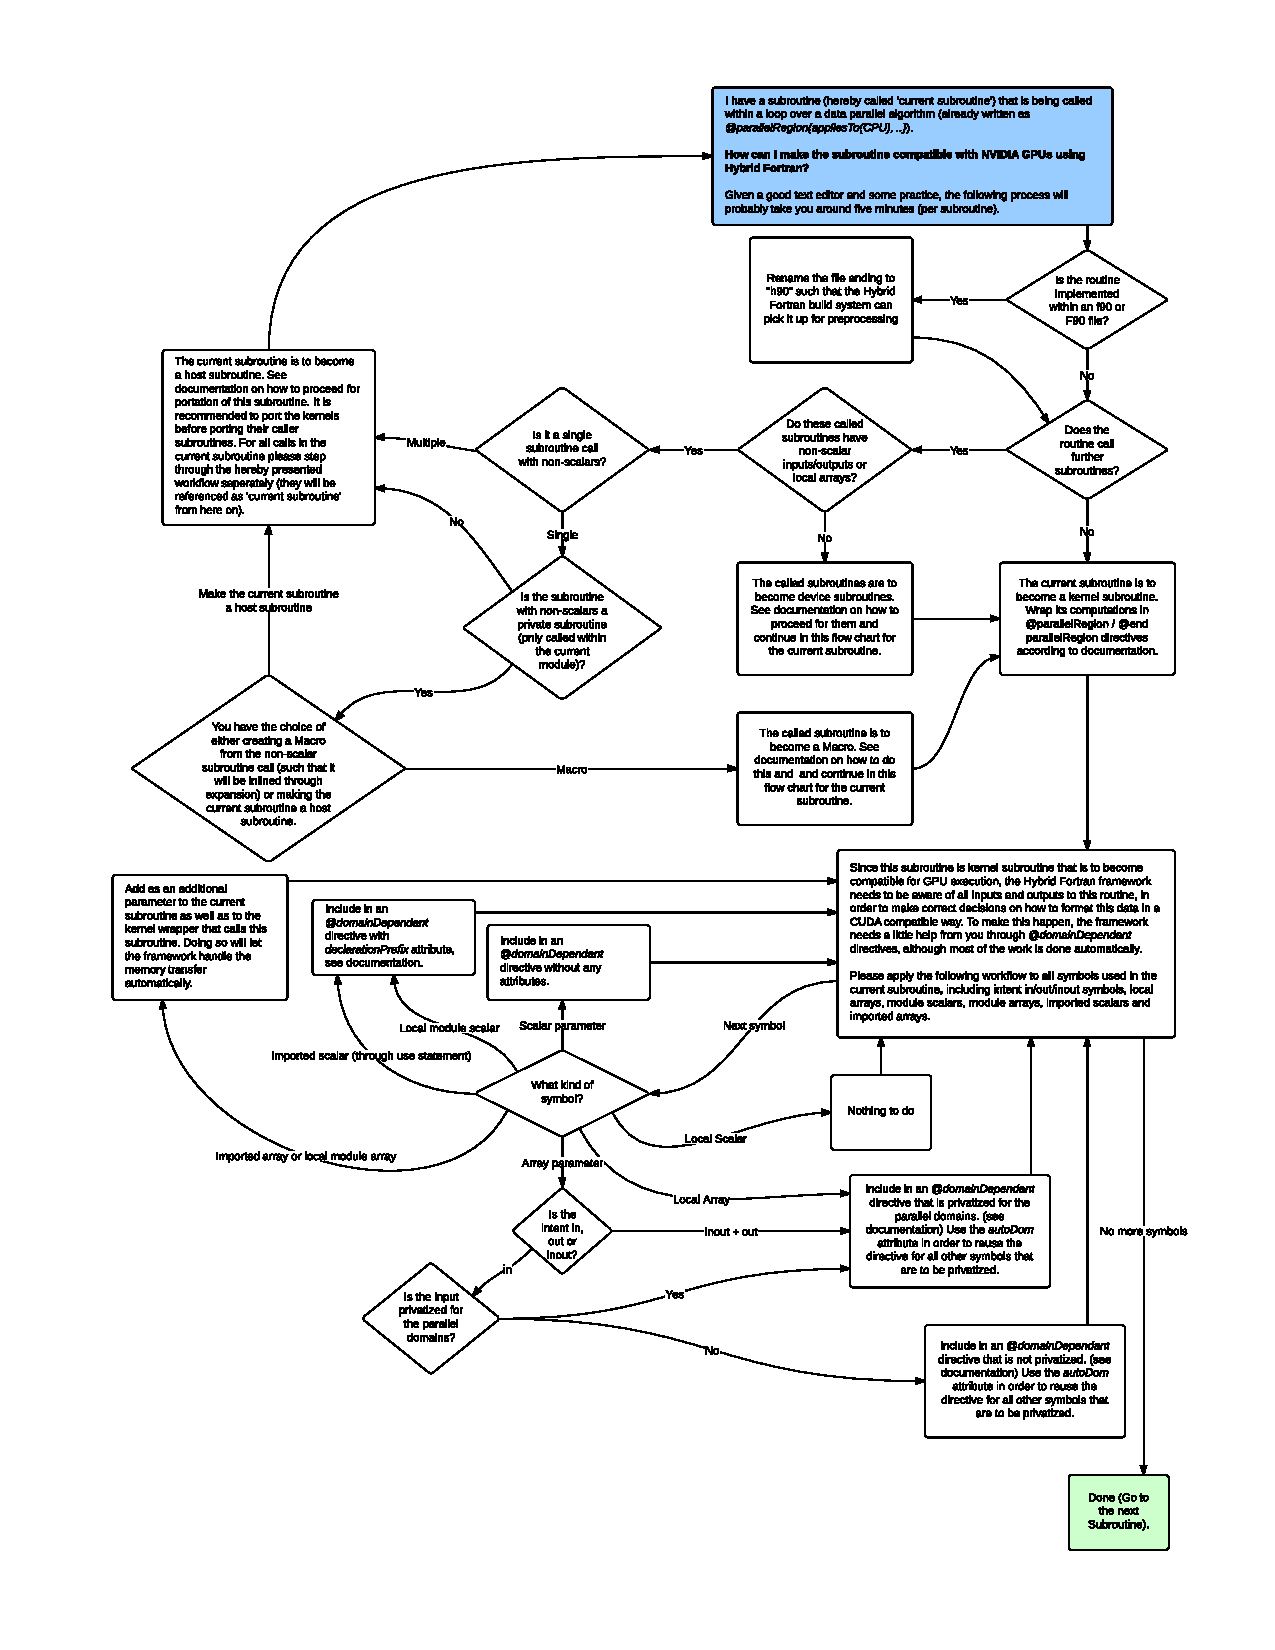
\includegraphics[width=16cm]{figures/HybridFortranGPUCompatibleCode.pdf}
  \caption [Best practices source code migration]{Best practices for a source code migration to Hybrid Fortran}
  \label{figure:bestPractMigration}
\end{figure}

Assuming that the starting point is a Fortran 90 source code for CPU, use the following guidance in order to port your codebase to \textbf{Hybrid Fortran} with the CUDA Fortran Backend. Please note: If you have many tight parallel loops in the same subroutine, you may want to start with the OpenACC backend, since it allows multiple parallel regions per subroutine. You can at a later point still easily migrate to the CUDA Fortran backend by splitting up your kernels into their own subroutine, if you find the OpenACC performance to be poor.

\begin{enumerate}
 \item Run \verb|make example| in the Hybrid Fortran root directory.
 \item Rename the new example project directory to your project name. You can also move it to any location you'd like.
 \item Delete \verb|source/example.h90| and copy in the sourcecode you'd like to hybridize using Hybrid Fortran. Please note that all loops that are to be run in parallel on CPU or GPU and their entire callgraph should be visible to the compiler in the source subdirectory. Your hybrid sources may be in an arbitrary subdirectory structure below the \verb|source| directory and may consist of \verb|f90| and \verb|F90| files. The buildsystem will find all your sourcefiles recursively and copy them into the respective build directory in a flat hierarchy.
 \item When it comes to integrating your hybrid sourcecode into a larger codebase, there are essentially two recommended options.
   \begin{enumerate}
     \item \label{enum:entireCodebase} Move the entire codebase over into the Hybrid Fortran build system. This is recommended if your build dependencies are specified in (or can easily ported to) one central Makefile.
     \item \label{enum:partOfFramework} (new since version 0.9) Move one (or later more) module of your sourcebase over into the Hybrid Fortran build system. In this case it is recommended to create a separate source directory for hybrid sources, move your code there and link its path using the \verb|SRC_DIR_COMMON| setting in \verb|MakesettingsGeneral|. Then, specify your other framework source directories using the setting \verb|FRAMEWORK_DIRS| and specify your previous main Makefile using the setting \verb|FRAMEWORK_MAKEFILE|. You should use the Makefile coming with Hybrid Fortran in the root project folder in order to interface with your build (no changes should be required other than the settings you specify in \verb|MakesettingsGeneral|. This will create separate build directories for the CPU and GPU case, copy in your \verb|FRAMEWORK_DIRS|, generate and compile the hybrid sources and then call \verb|FRAMEWORK_MAKEFILE| within the build directory. You will also need the settings \verb|FRAMEWORK_EXECUTABLE_PATHS| and \verb|FRAMEWORK_INSTALLED_EXECUTABLE_PATHS| in order to tell Hybrid Fortran which executables are being created by your build system and where you'd like them installed afterwards for testing purposes. You will need to adapt your previous build system for having moved your hybrid sources.
   \end{enumerate}
 \item In case you went with option \ref{enum:entireCodebase}, adapt your filenames containing main routines. The filename of your file(s) containing main routines need to correspond to the executable names you have specified in the \verb|EXECUTABLES| variable in \verb|MakesettingsGeneral|. E.g. if you want executables named \verb|production_exec|, \verb|test1_exec| and \verb|test2_exec|, the corresponding main files need to be named \verb|production_exec.f90|, \verb|test1_exec.f90| and \verb|test2_exec.f90|.
 \item Adjust \verb|config/MakesettingsGeneral| - the configuration options should be self explanatory.
 \item Adjust \verb|config/Makefile| by adding your hybrid source dependencies (and deleting the example). If your previous build system was already built on \verb|GNU Make| it should be possible to cut and paste your dependency definitions without change. If you would like to exclude some files or folders in your source directory from compilation (in order to integrate modules one by one), you can do this by editing the \verb|EXCEPTIONS| variable in \verb|MakesettingsGeneral|.
 \item Adjust the \verb|FFLAGS| and \verb|LDFLAGS| variables in \verb|config/MakesettingsGPU| and \verb|config/MakesettingsCPU| to reflect the compiler and linker options that are needed to compile your codebase. Please note that currently only CUDA Fortran with the Portland Group compiler \verb|pgf90| is supported and tested as the GPU implementation.
 \item Adjust the \verb|source/storage_order.F90| file according to the comments you find there. This defines storage order macros and a few other variables that Hybrid Fortran will use at the preprocessor stage. Make sure that the storage order matches a scheme that is performant on the respective target architecture - as the example shows, the \verb|GPU| variable can be used to differentiate between GPU and CPU architecture. For the GPU case, the first dimension should be the one that gets mapped to X on the threadblocks, in order for memory accesses to be coalesced. This is in turn the first dimension you specify in the \verb|domName| and \verb|domSize| attributes in your \verb|@parallelRegion| directives.
 \item Run \verb|make; make install| and run your program in order to test whether the integration of your sourcecode into the \textbf{Hybrid Fortran} build system has been successful. It should create the cpu and gpu executable versions of your program in the test directory, however the gpu version will not run on the GPU yet, since no directives have been defined so far.
 \item Integrate a test system. You can use the test scripts that have been provided with this framework (see sec.~\ref{sec:testSystem}) or use any other test system.
 \item Define the parallel regions that are to be accelerated by CPU\footnote{For example ``do'' loops that are already executed on multicore CPU using OpenMP statements.} using a \linebreak\verb|@parallelRegion{appliesTo(CPU), ...}| directive. See sec.~\ref{sub:parallelRegionDirective} for details. Rename all files that (a) contain such regions or (b) contain subroutines that are part of the call hierarchy inside those regions from \verb|*.f90| or \verb|*.F90| to \verb|*.h90|.
 \item Make sure your program still compiles and runs correctly on CPU by executing \verb|make clean; make install_cpu; [run your tests]|.
 \item (optional, you will need graphviz and pydot) Run \verb|make graphs|. You should now have a graphical representation of your call hierarchy as ``seen'' from your parallel regions upwards and downwards in the call tree.
 \item Define the subprocedures within that call hierarchy that are to be ported as GPU kernels. Fig.~\ref{figure:bestPractMigration} is designed to help you with that process. Kernel subprocedures should have the following properties:
  \begin{enumerate}
   \item They only call subprocedures from the same module.
   \item They only call one more level of subprocedures (rule of thumb).
   \item The set of these subprocedures is self enclosed for all data with depencies in your parallel domains, i.e. your data is only directly read or written to inside these to-be kernels and their callees. If this is not the case it will be necessary to restructure your codebase, e.g. put pre- and postprocessing tasks that are defined inline within higher level subprocedures into subprocedures and put them into your set of kernels.
  \end{enumerate}
 \item Make sure that callgraphs within GPU kernel subprocedures as well as kernel subprocedure callers are all defined in h90/H90 files (rename from f90/F90 where necessary).
 \item Make sure that at least the kernel callers have all the array arguments defined using \verb|intent| statements (\verb|in, out, inout|). It is recommended that all arguments in all your subroutines are defined this way, since the compiler will pick up some logical errors for you with this information. This includes pointer types as well.
 \item Analyse for all kernels which data structures they require and which of those structures are dependant on your parallel domain. Define \verb|@domainDependant| directives for those data structures within all kernels, kernel subprocedures and all intermediate subprocedures between your kernels and your CPU parallel region. See sec.~\ref{sec:archDirectives} for details. In kernel subroutines and inside kernel subroutines you will need to declare local scalars and imported data as well. See sec.~\ref{sub:domainDependantDirective} for details. See also fig.~\ref{figure:bestPractMigration}.
 \item If your kernels use arrays from the local module or imported arrays, pass them to the kernel subroutine using parameters. Use appropriate \verb|@domainDependant| directives. See sec.~\ref{sub:domainDependantDirective} for details.
 \item Imported arrays that are used in kernel subroutines and inside kernel subroutines also need to be input parameters of the kernel caller itself for appropriate automatic device data handling. That is, they need to be passed down to the kernels on two levels. Use appropriate \verb|@domainDependant| directives.
 \item Wrap the implementation sections of all your kernels with \linebreak\verb|@parallelRegion{appliesTo(GPU), ...}| / \verb|@end parallelRegion| directives. See sec.~\ref{sub:parallelRegionDirective} for details.
 \item Test and debug on CPU by executing \linebreak\verb|make clean;make build_cpu DEBUG=1| with automatic tests enabled. You can use any compatible x86 debugger here, such as PGI debugger, Intel debugger, Totalview or Allinea DDT. Please note that the debuggers will show you the line numbers of the respective \verb|F90| files, not your \verb|h90| or \verb|H90| files. The \verb|F90| files have been kept as readable as possible however, and they can all be inspected in \verb|./build/cpu/source|. Fig.~\ref{figure:bestPractDebugging} is designed to help you with this process.
 \item Switch to GPU tests debug on GPU using \linebreak\verb|make clean;make build_gpu DEBUG=1; make install_gpu; [run your tests]|. Fig.~\ref{figure:bestPractDebugging} is designed to help you with this process. The print output will help you identify problems that only exist in the GPU version. Hint: Most of the bugs that persist after having a correct CPU implementation are usually related to data dimensionalities specified using \verb|@domainDependant| directives. You should be able to trace back the error by comparing the printed output with the CPU version opened in a separate debugger window and thus identify the kernels responsible for the errors. Once you've found the offending kernels, make sure the data is correctly formatted in the specification part of the \verb|F90| file in \verb|./build/gpu/source|. If the printed output does not show the error (whose index point should be recognized in your validation / test system you've integrated before), you can change the debug data indexes in \verb|storage_order.F90|.
 \item Congratulations, you have just completed a CPU/GPU hybrid portation using \textbf{Hybrid Fortran}.
\end{enumerate}

\begin{figure}[hbtp]
  \centering  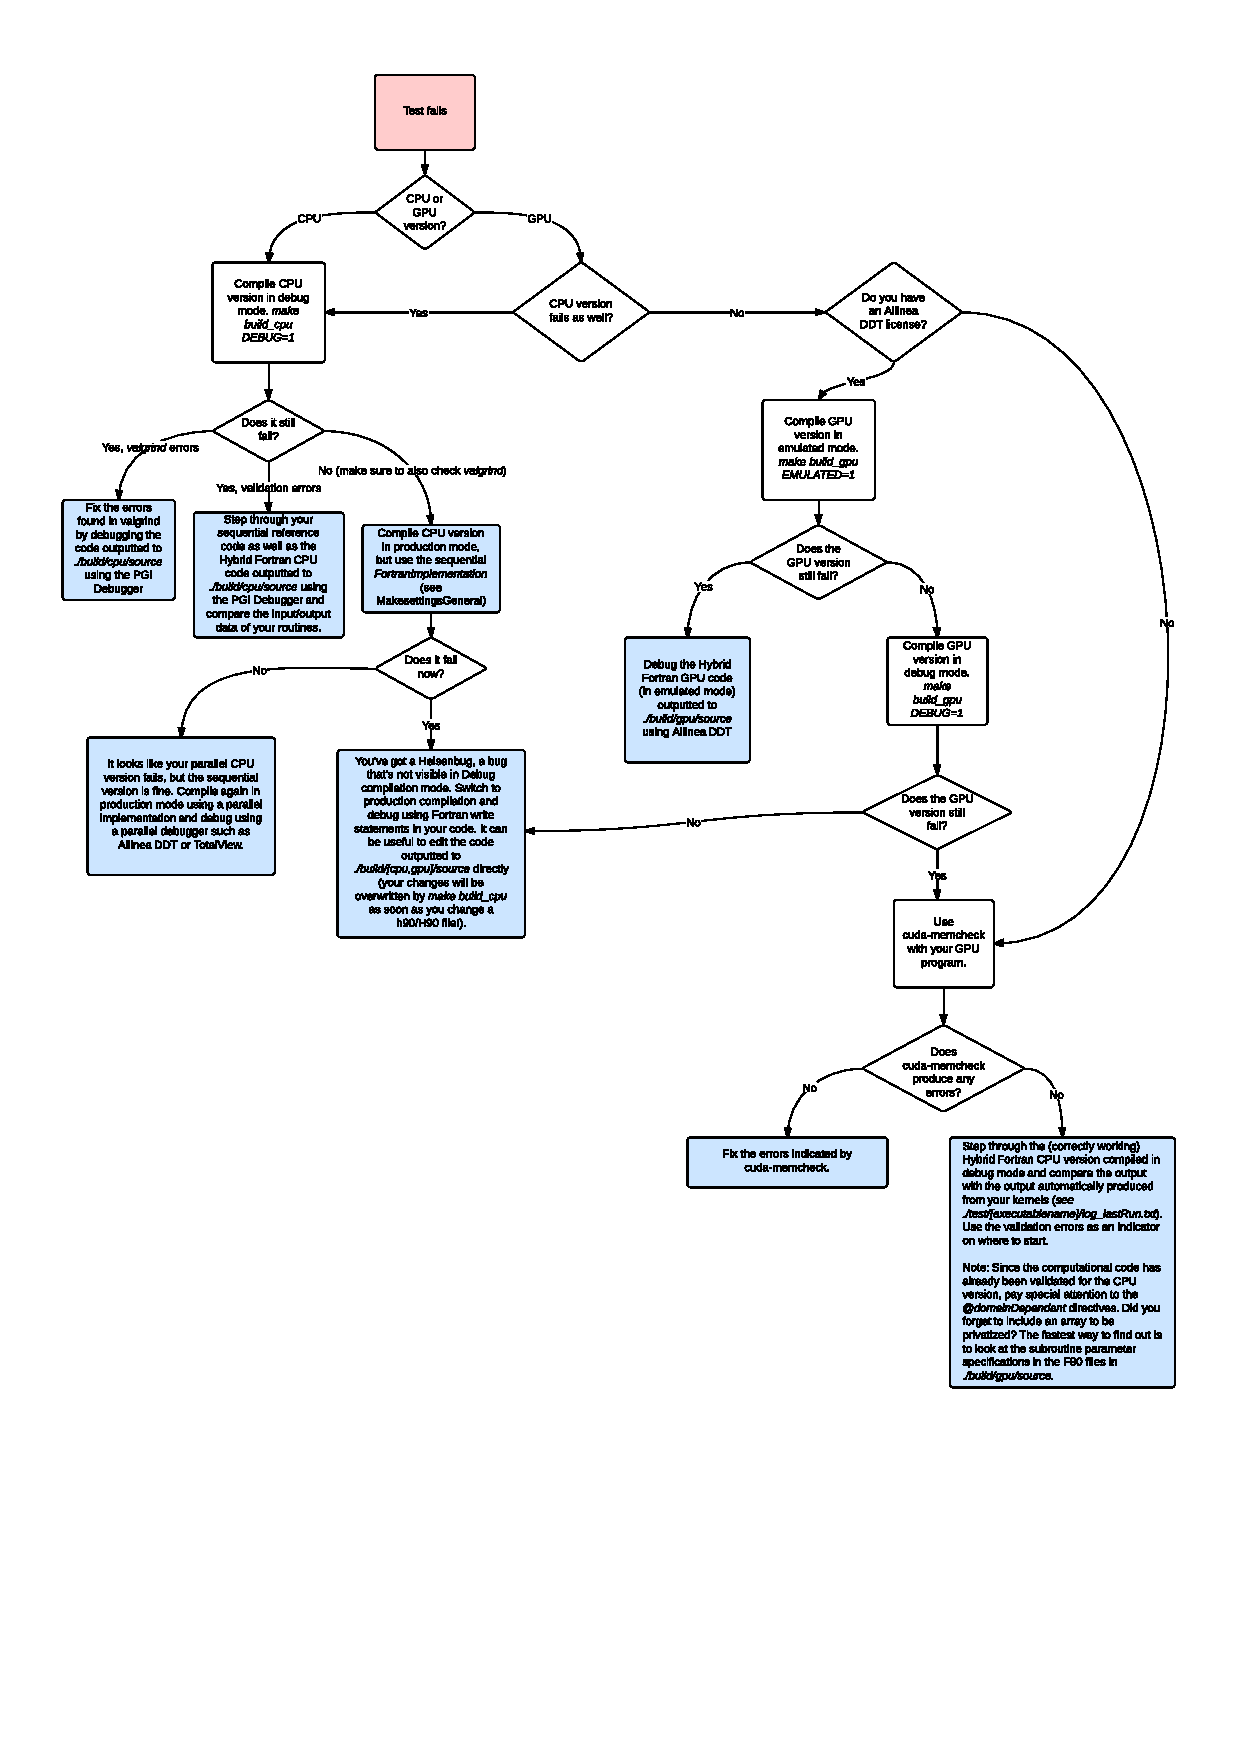
\includegraphics[width=16cm]{figures/HybridFortranDebugging.pdf}
  \caption [Best practices debugging]{Best practices for debugging Hybrid Fortran code}
  \label{figure:bestPractDebugging}
\end{figure}



\clear
\chapter{Framework Implementation} \label{cha:implementation}
In this chapter the design of the \textbf{Hybrid Fortran} framework is presented from the implementation perspective. It will discuss the architecture that has been introduced for implementing the \textbf{Hybrid Fortran} framework, in order to achieve the goals and behaviour outlined in sec.~\ref{sec:frameworkGoals} and sec.~\ref{sec:archDirectives}. If you'd like to adjust the framework for your own purposes, this chapter is a good place to start.

\section{Overview and Build Workflow} \label{sub:buildSystem}

\begin{figure}[htpb]
	\centering
	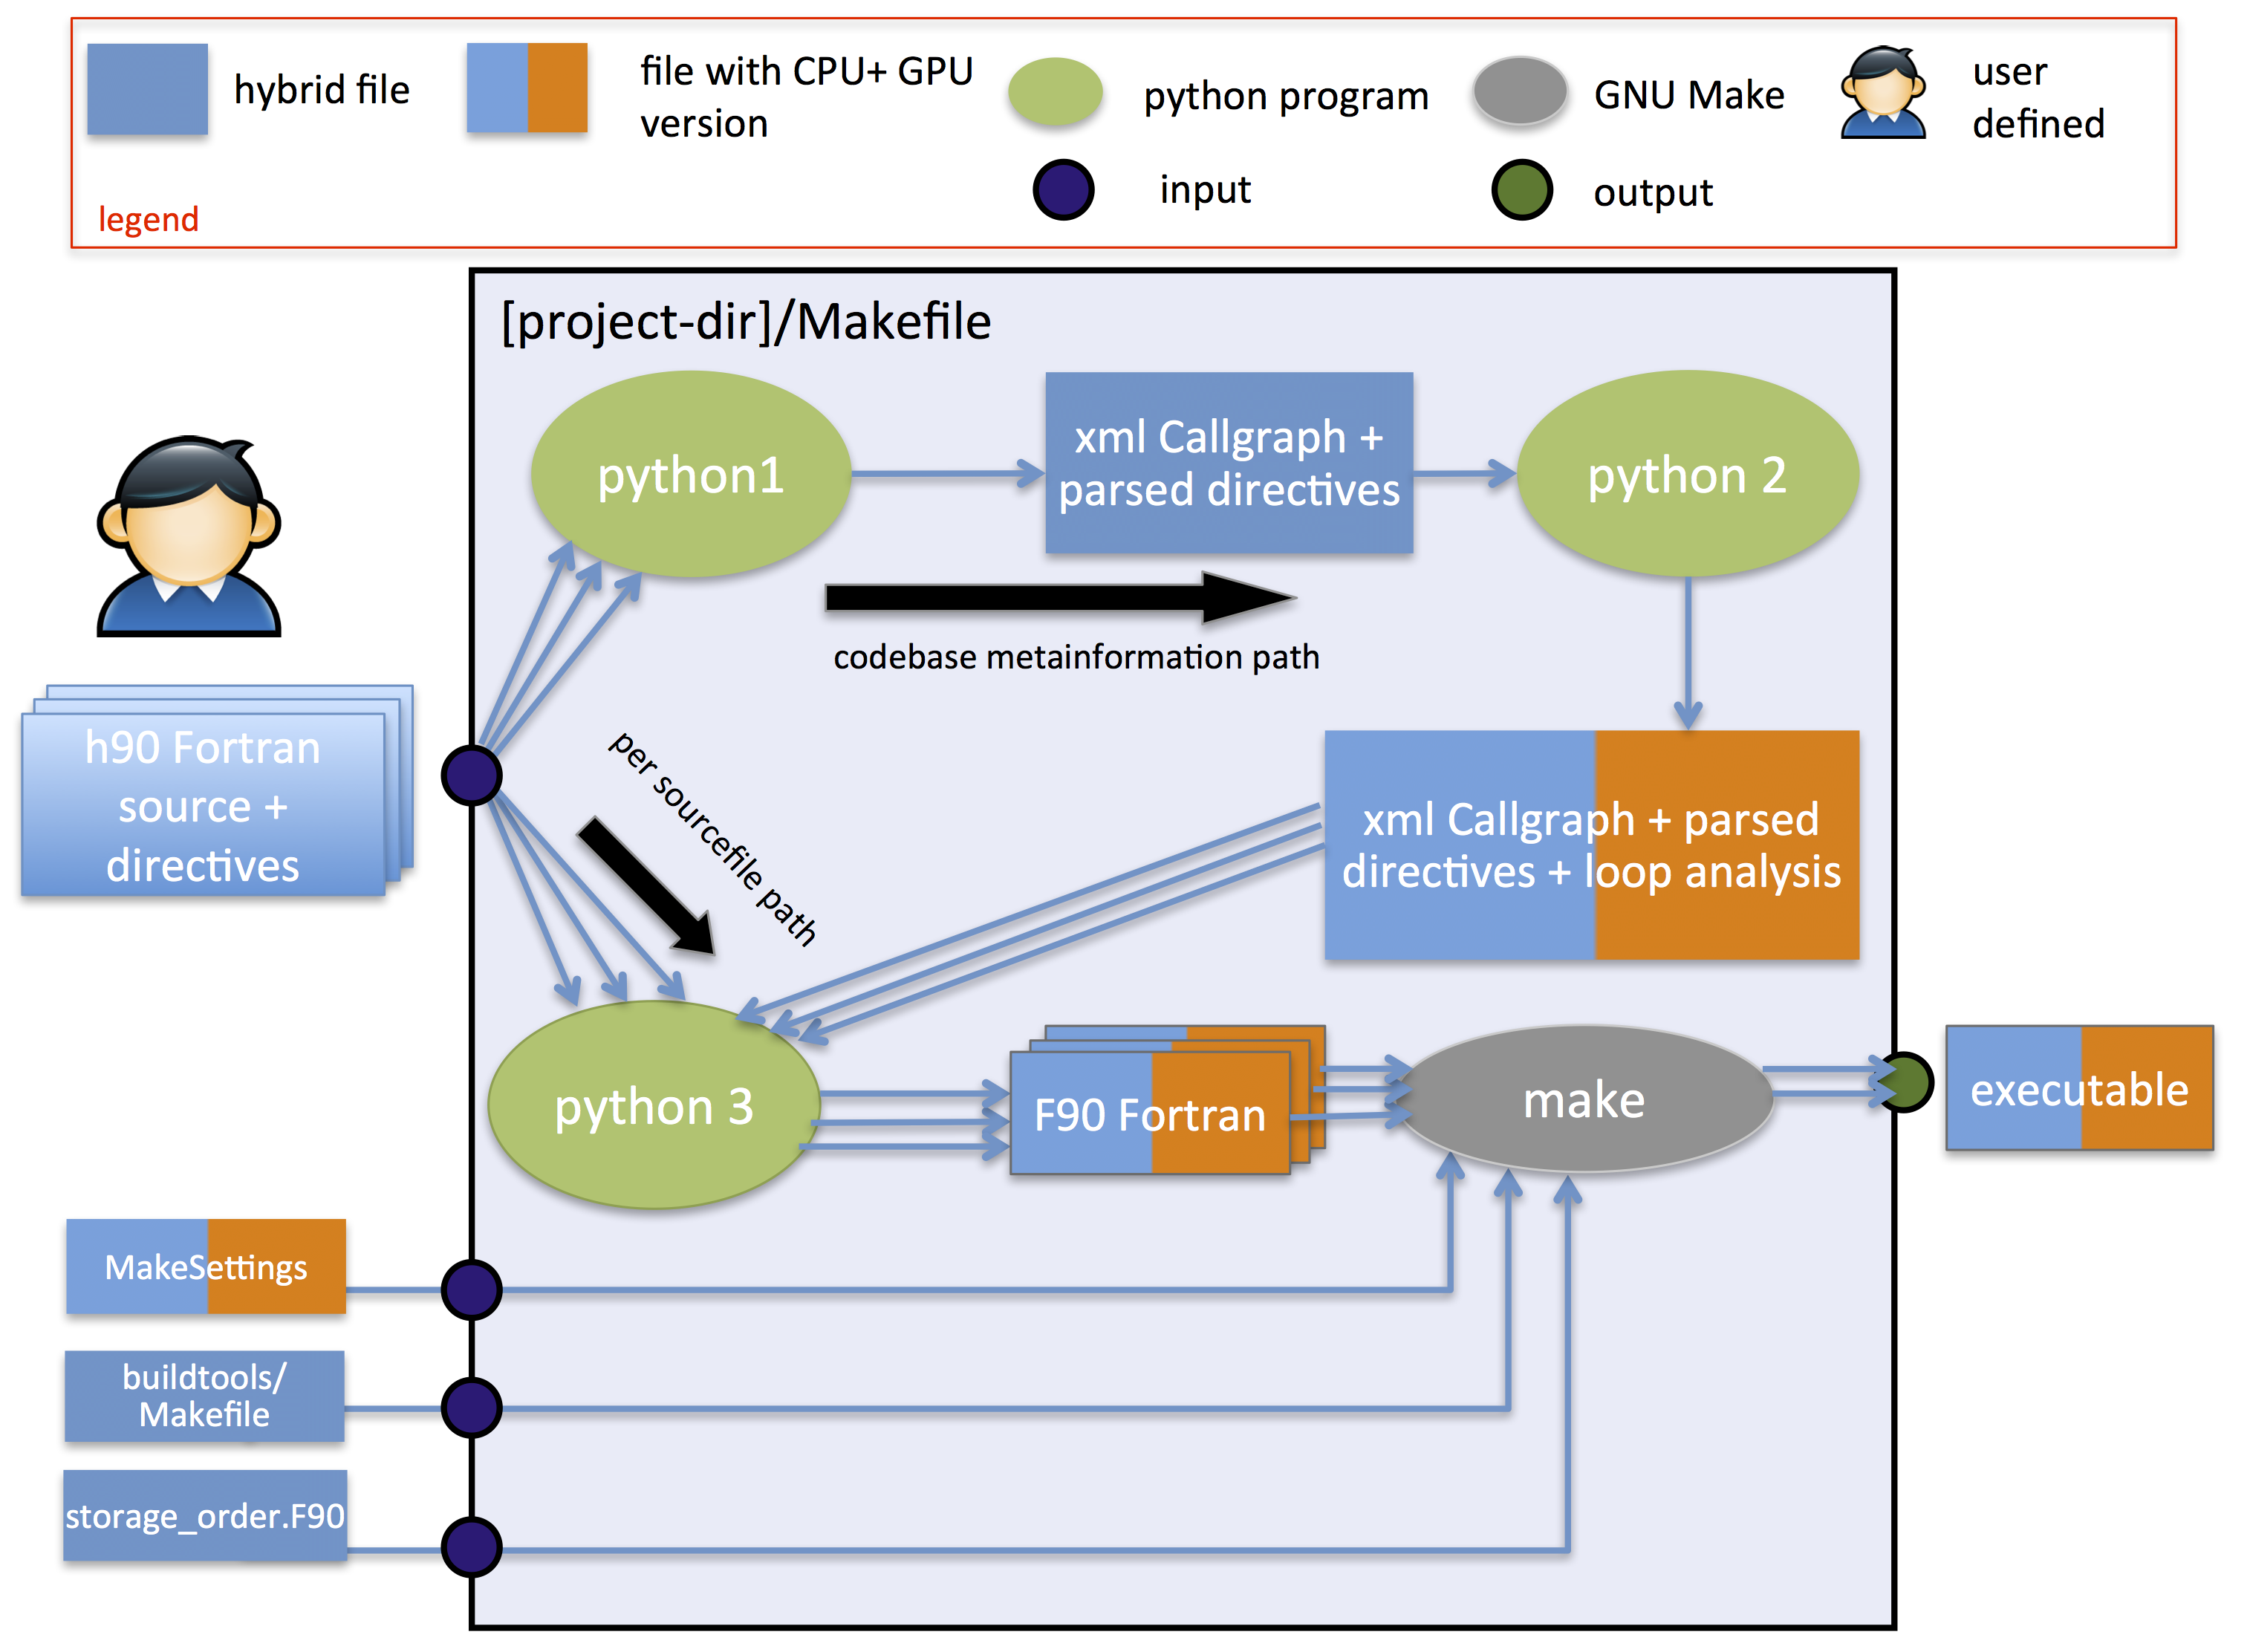
\includegraphics[width=14cm]{figures/hybridCUDAInformationFlow}
	\caption[Hybrid Fortran Components]{\textbf{Hybrid Fortran} Components and Information Flow.}
	\label{figure:hybridCUDAComponentsAndInfoFlow}
\end{figure}

The \textbf{Hybrid Fortran} build system involves the following components (depicted in fig.~\ref{figure:hybridCUDAComponentsAndInfoFlow}):

\begin{description}
 \item[project-dir/Makefile] offers a convenient interface to the build system. Please refer to appendix \ref{sub:buildInterface} for the usage of this build interface. It performs the following operations (assuming a clean rebuild):
 \begin{enumerate}
  \item Creates a build directory containing subdirectories for CPU and GPU builds.
  \item Copies all \verb|f90| and \verb|F90| source files (pure Fortran 90 sources without \textbf{Hybrid Fortran} directives) into the CPU and GPU build directories using a flat file hierarchy.
  \item Creates the callgraph \verb|xml| file as well as the colored CPU and GPU callgraph versions in the callgraph subdirectory within the build directory.
  \item Creates the graphical callgraph representations in the callgraph directory using \textbf{Graphviz} libraries.
  \item Converts each \verb|h90| source file into \verb|F90| source files, using different implementations and callgraph colorings for the CPU and GPU case. The \verb|F90| files are created in their respective build subdirectories (CPU or GPU).
  \item Copies the \verb|project-dir/buildtools/Makefile| into the CPU and GPU source directories.
  \item Copies either \verb|project-dir/buildtools/MakesettingsCPU| and \linebreak
    \verb|project-dir/buildtools/MakesettingsGPU| into the respective build subdirectory.
  \item Executes \verb|make| within the build subdirectories.
  \item Installs the resulting executables into the test directory, using \verb|cpu| or \verb|gpu| as a postfix in the executable filename.
 \end{enumerate}
 \item[project-dir/buildtools/Makefile] defines the dependencies between the Fortran 90 and \textbf{Hybrid Fortran} sources.
 \item[project-dir/buildtools/MakesettingsCPU] defines the compiler name, compiler flags and linker flags for the CPU case.
 \item[project-dir/buildtools/MakesettingsGPU] defines the compiler name, compiler flags and linker flags for the GPU case.
\end{description}

\begin{figure}[htpb]
	\centering
	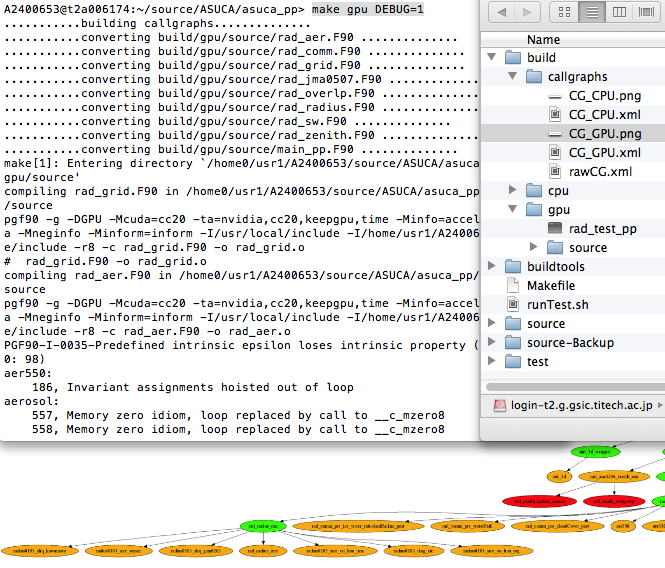
\includegraphics[width=10cm]{figures/uiScreenShot}
	\caption[Screenshot Build System]{Screenshot of the \textbf{Hybrid Fortran} build system in action.}
	\label{figure:buildSystemInAction}
\end{figure}

\section{Python Build Scripts} \label{sub:pythonScripts}

\noindent The following python command line interface programs are part of the \textbf{Hybrid Fortran} build system:

\begin{description}
 \item[annotatedCallGraphFromH90SourceDir.py] goes through all h90 files in a given source directory and builds an xml file containing meta information about that source tree. The extracted meta information includes the callgraph visible from h90 files as well as a parsed version of the \textbf{Hybrid Fortran} directives inserted by the user. Figure \ref{figure:hybridCUDAComponentsAndInfoFlow} depicts this program in node \verb|python 1|.
 \item[loopAnalysisWithAnnotatedCallGraph.py] takes the meta information xml file from the previous script as its input and analyses the positioning of the user defined parallel regions relative to all subprocedures. Depending on its input arguments it performs this analysis for either the CPU or GPU version of the program in order for the framework to support compile time defined positioning of loops (kernel regions in the CUDA implementation). Figure \ref{figure:hybridCUDAComponentsAndInfoFlow} depicts this program in node \verb|python 2|.
 \item[generateF90fromH90AndAnalyzedCallGraph.py] takes one h90 source file as well as the analyzed meta information xml file as its inputs. It goes through the source file line by line and rewrites it in order to create compatible versions for CPU and GPU. The following operations are most essential to this module:
 \begin{itemize}
  \item Rewriting of parallel region definitions to conventional loops for the CPU or CUDA Fortran kernels for the GPU.
  \item Mutation of declarations and accesses of domain dependant arrays according to their position relative to the currently active parallel region.
  \item Insertion of statements to copy array data to and from the device in the GPU case.
 \end{itemize}
 Parallel domain dependant Figure \ref{figure:hybridCUDAComponentsAndInfoFlow} depicts this program in node \verb|python 3|.
 \item[graphVizGraphWithAnalyzedCallGraph.py] This program has been created in order to make debugging easier and to give the user an overview over the codebase and the involved parallel regions. It creates a graphical representation of the call graph from the analyzed meta information. The nodes in these call graphs are colored according to their relative position to the parallel regions. Figure \ref{figure:callgraph} shows a sample of such a programmatically created call graph representation.
\end{description}

\begin{figure}[htpb]
	\centering
	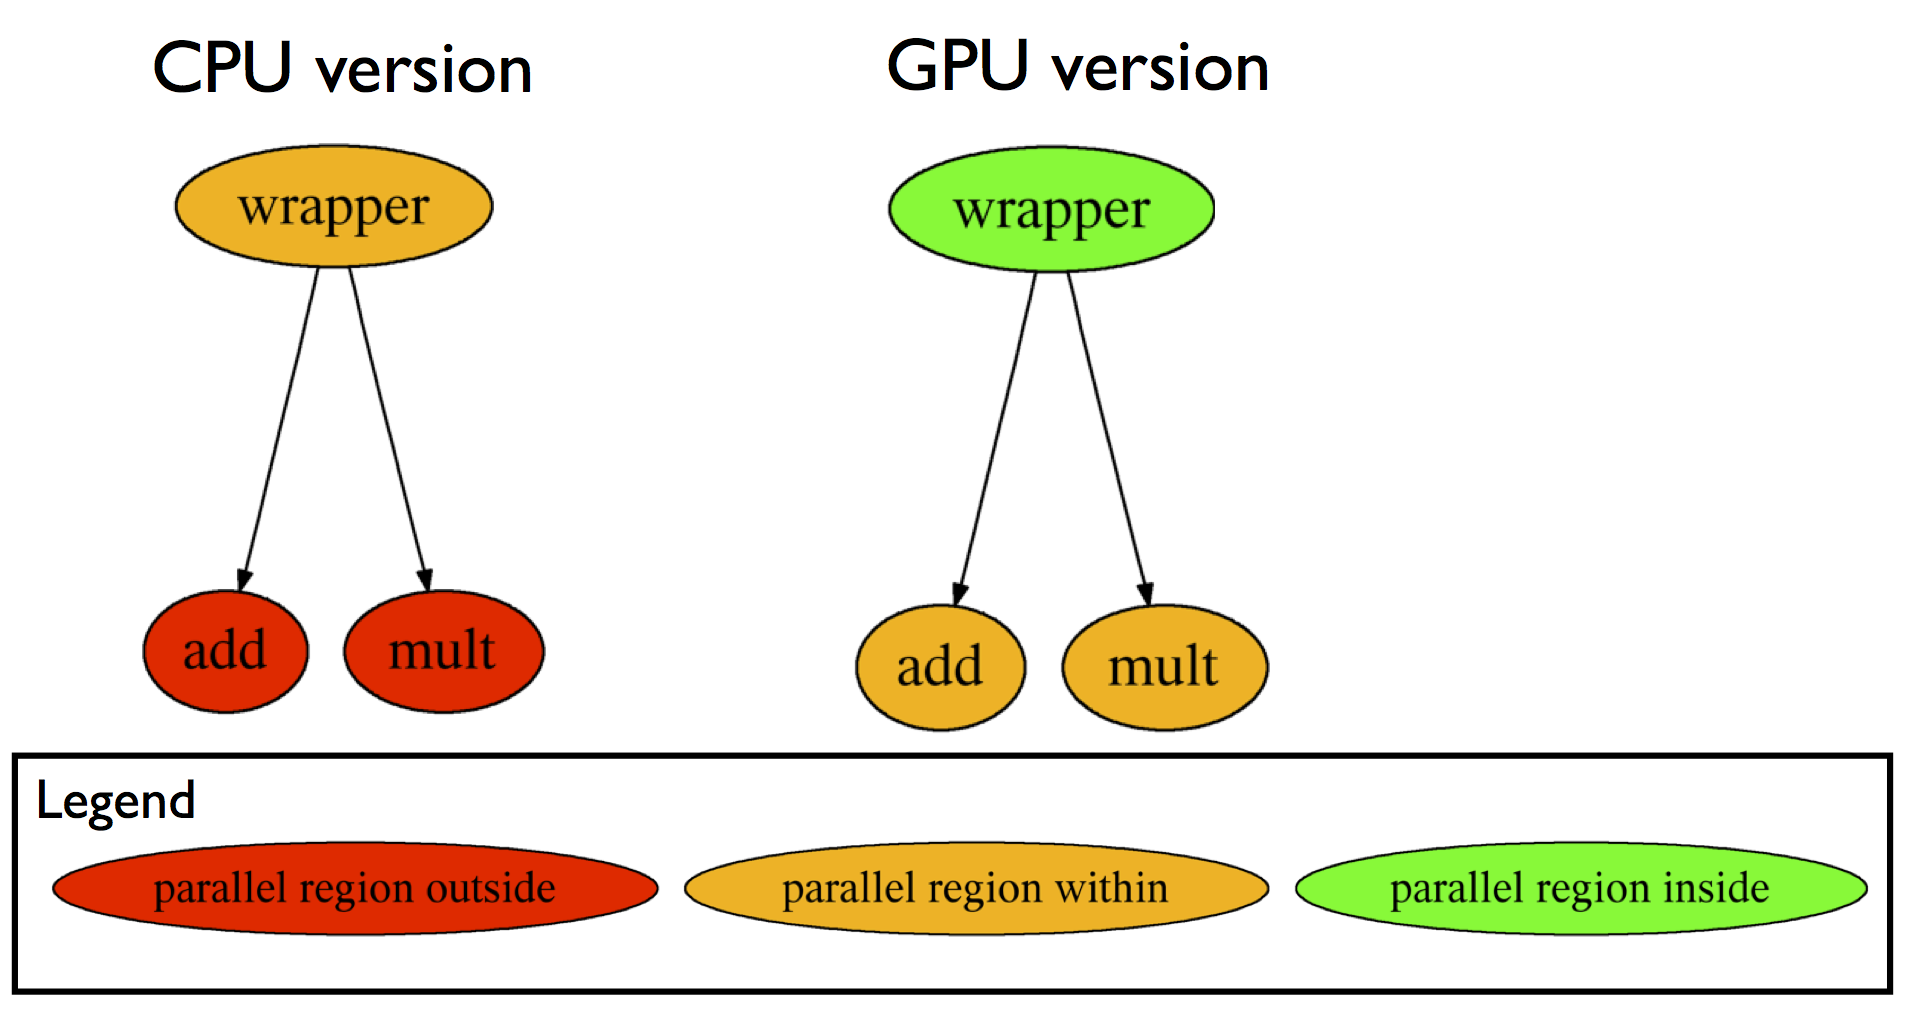
\includegraphics[width=10cm]{figures/callgraph}
	\caption[Callgraph Example]{Condensed version of a simple callgraph, programmatically created by graphVizGraphWithAnalyzedCallGraph.py.}
	\label{figure:callgraph}
\end{figure}

\section{User Defined Files} \label{sub:userDefinedFiles}

The following files, depicted figure \ref{figure:hybridCUDAComponentsAndInfoFlow}, are defined by the user:

\begin{description}
 \item[h90 Fortran sources] A source directory that contains \textbf{Hybrid Fortran} files (h90 extension). It may also contain files with f90 or F90 extensions. The source directory is by default located at \verb|path-to-project/source/*|.
 \item[Makefile] Used to define module dependencies. The Makefile is by default located at \verb|path-to-project/buildtools/Makefile|. Note: All source files are being copied into flat source folders before being compiled - the build system is therefore agnostic to the source directory structure implemented by the framework user.
 \item[storage\_order.F90] This fortran file contains fortran preprocessor statements in order to define the storage order for both CPU and GPU implementation. This file is located at
 \begin{verbatim*}path-to-project/source/
hybrid_fortran_commons/storage_order.F90.\end{verbatim*}

\end{description}

\section{Class Hierarchy} \label{sub:archHierarchy}

\begin{figure}[htpb]
	\centering
	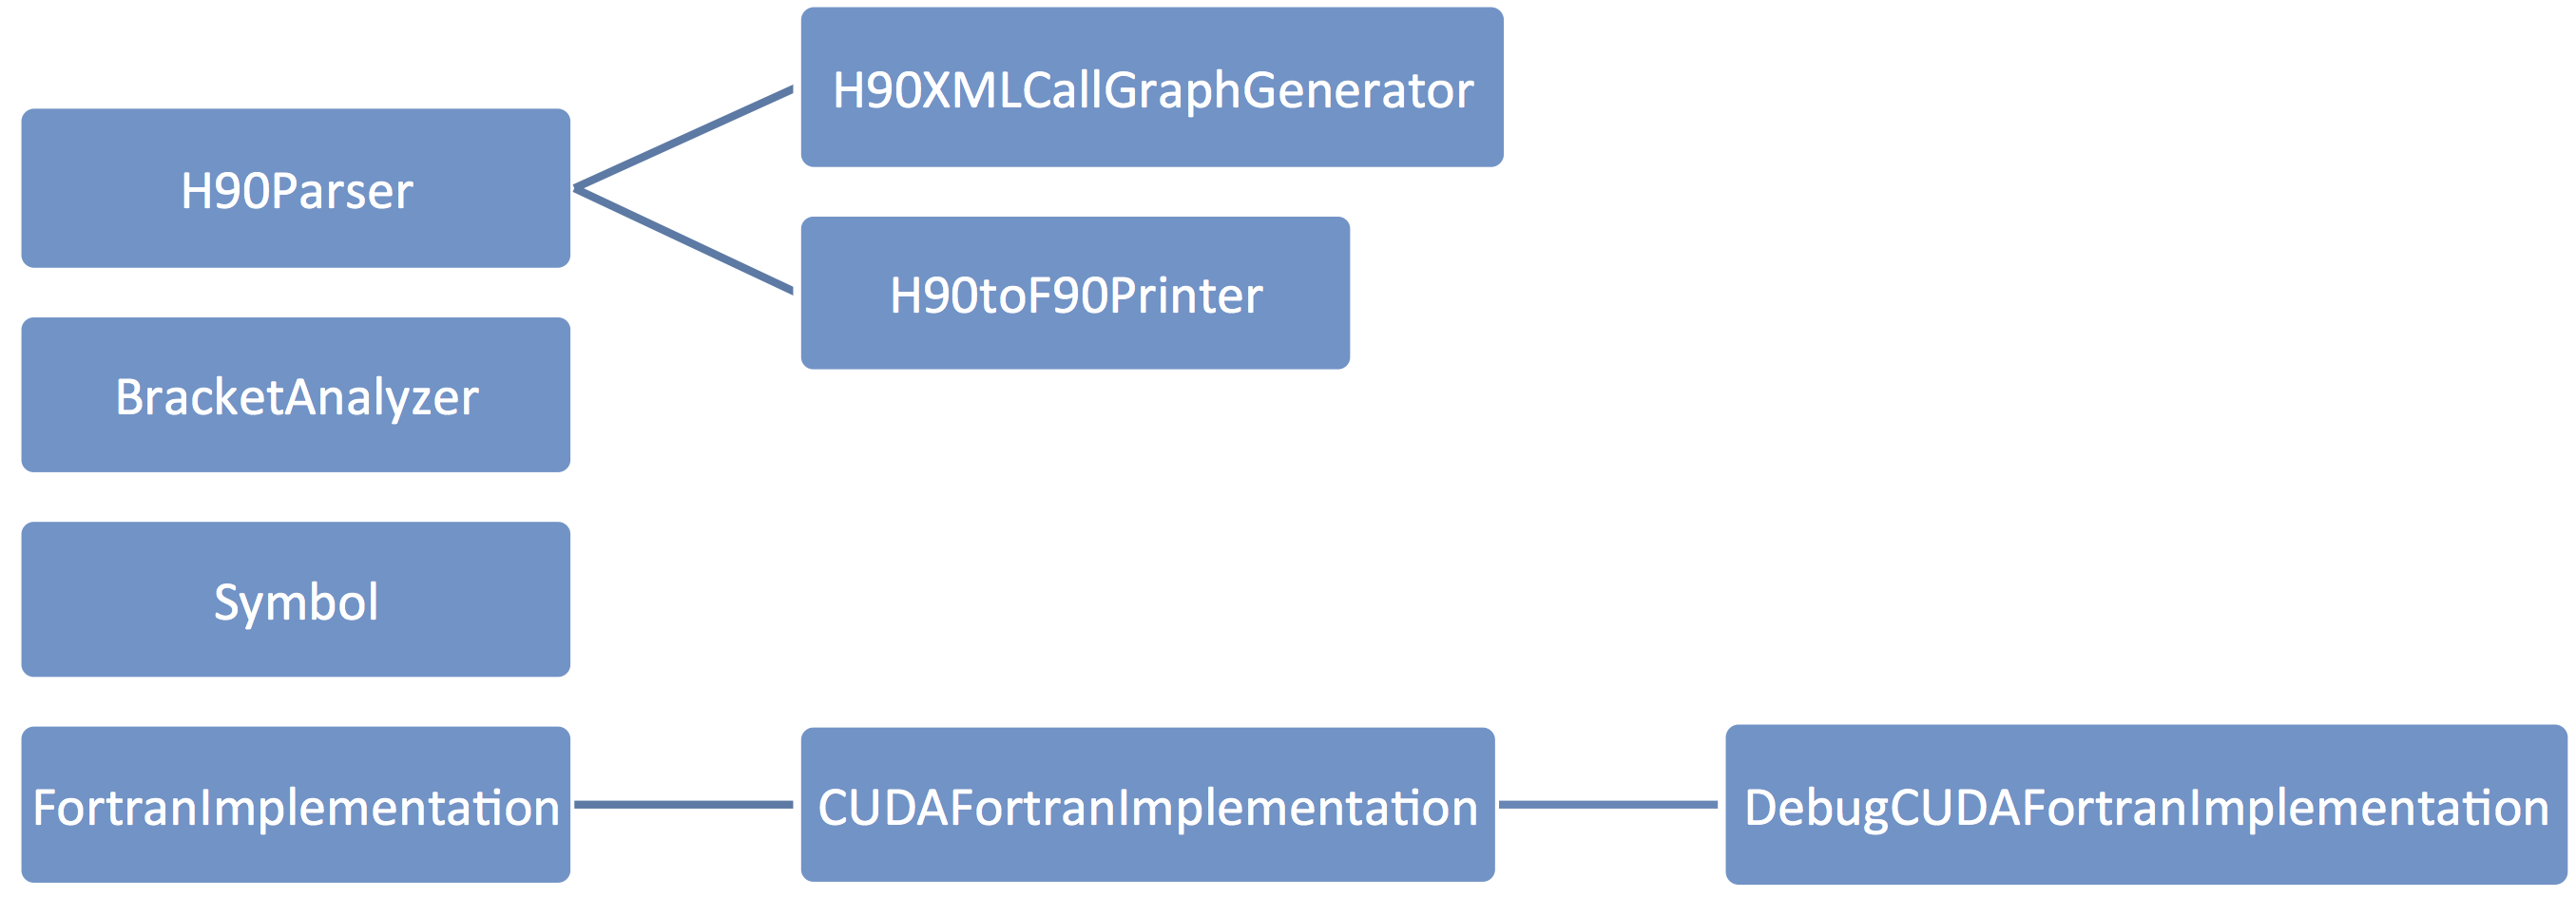
\includegraphics[width=14cm]{figures/classHierarchy}
	\caption[Hybrid Fortran Python Class Hierarchy]{\textbf{Hybrid Fortran} Python Class Hierarchy.}
	\label{figure:classHierarchy}
\end{figure}

Figure \ref{figure:classHierarchy} shows the classes created to implement the functionality described in section \ref{sub:pythonScripts}. For a full list of the implementation classes, please see also sec. \ref{sub:backendImplementation}.

\begin{description}
 \item[H90Parser] parses \textbf{Hybrid Fortran} (h90) files. The parser uses a mixture of state machine and regular expression design patterns. More specifically: Each line is matched against a set of regular expressions. The set of regular expressions being used is determined by a state machine and the outcomes of the regular expression matches in turn determine the state transitions.
 See section \ref{sub:parser} for a more detailed look at the \textbf{Hybrid Fortran} parser implementation.
 \item[H90XMLCallGraphGenerator] (subclass of \verb|H90Parser|) adds routine and call nodes to a new or existing call graph xml document. This functionality is used by \linebreak
 \verb|annotatedCallGraphFromH90SourceDir.py| as described in section \ref{sub:pythonScripts}.
 \item[H90toF90Converter] (subclass of \verb|H90Parser|) prints a fortran 90 file in F90 format (including preprocessor statements) to POSIX standard output. The configuration of this class includes
  \begin{enumerate}
    \item a \textbf{Hybrid Fortran} file as its main input (inherited from the parent class).
    \item an xml callgraph including parsed \textbf{Hybrid Fortran} directives and the positions of parallel regions relative ot the routine nodes.
    \item a FortranImplementation object which determines the parallel implementation.
  \end{enumerate}
  \verb|generateF90fromH90AndAnalyzedCallGraph.py| uses this functionality as described in section \ref{sub:pythonScripts}.
 \item[BracketAnalyzer] is used to determine whether a Fortran line ends with an open bracket.
 \item[Symbol] Stores array dimensions determined at the time of declaraton for later use and includes functionality to print adapted declaration and access statements.
 \item[FortranImplementation] provides the concrete syntax for a standard Fortran 90 implementation of the \textbf{Hybrid Fortran} program.
 \item[CUDAFortranImplementation] (subclass of \verb|FortranImplementation|) provides the syntax for a CUDA Fortran implementation, thus handling
 \begin{itemize}
  \item the conversion of parallel region directives into CUDA kernels,
  \item the conversion of subroutines called by kernels into device subroutines,
  \item the copying of data from and to the device,
  \item the synchronization of threads after CUDA kernels have finished executing (asynchronous execution of kernels is currently not supported) and
  \item error handling.
 \end{itemize}
 \item[DebugCUDAFortranImplementation] (subclass of \verb|CUDAFortranImplementation|) extends the CUDA Fortran implementation to include print statements to POSIX standard error output for all kernel parameters at a user defined data point after the execution of the kernel. This functionality enables debugging of device code since barebone CUDA Fortran currently does not offer printing or debugging for code executed on the GPU. (There is an emulation mode available which runs CUDA Fortran programs on the CPU, however it has been found to diverge too much from the device version).
\end{description}

\section{Switching Implementations} \label{sub:switchImplementation}

Figure \ref{figure:implementationMap} shows the the most important class member functions of \linebreak
\verb|FortranImplementation| classes and their role with respect to the example shown earlier in section \ref{sub:directiveExample}. Each of these methods takes context information objects (for example a set of symbols that are referenced on this line, or a parallel region template containing the information users have passed with the directives) and returns strings that will be inserted at the indicated places into Fortran 90 files by the \verb|H90toF90Converter| class. Introducing a new underlying technology such as OpenCL (for GPU implementations) or OpenMP (for CPU implementations) is as simple as writing a new \verb|FortranImplementation| subclass containing these functions.

\begin{figure}[htpb]
	\centering
	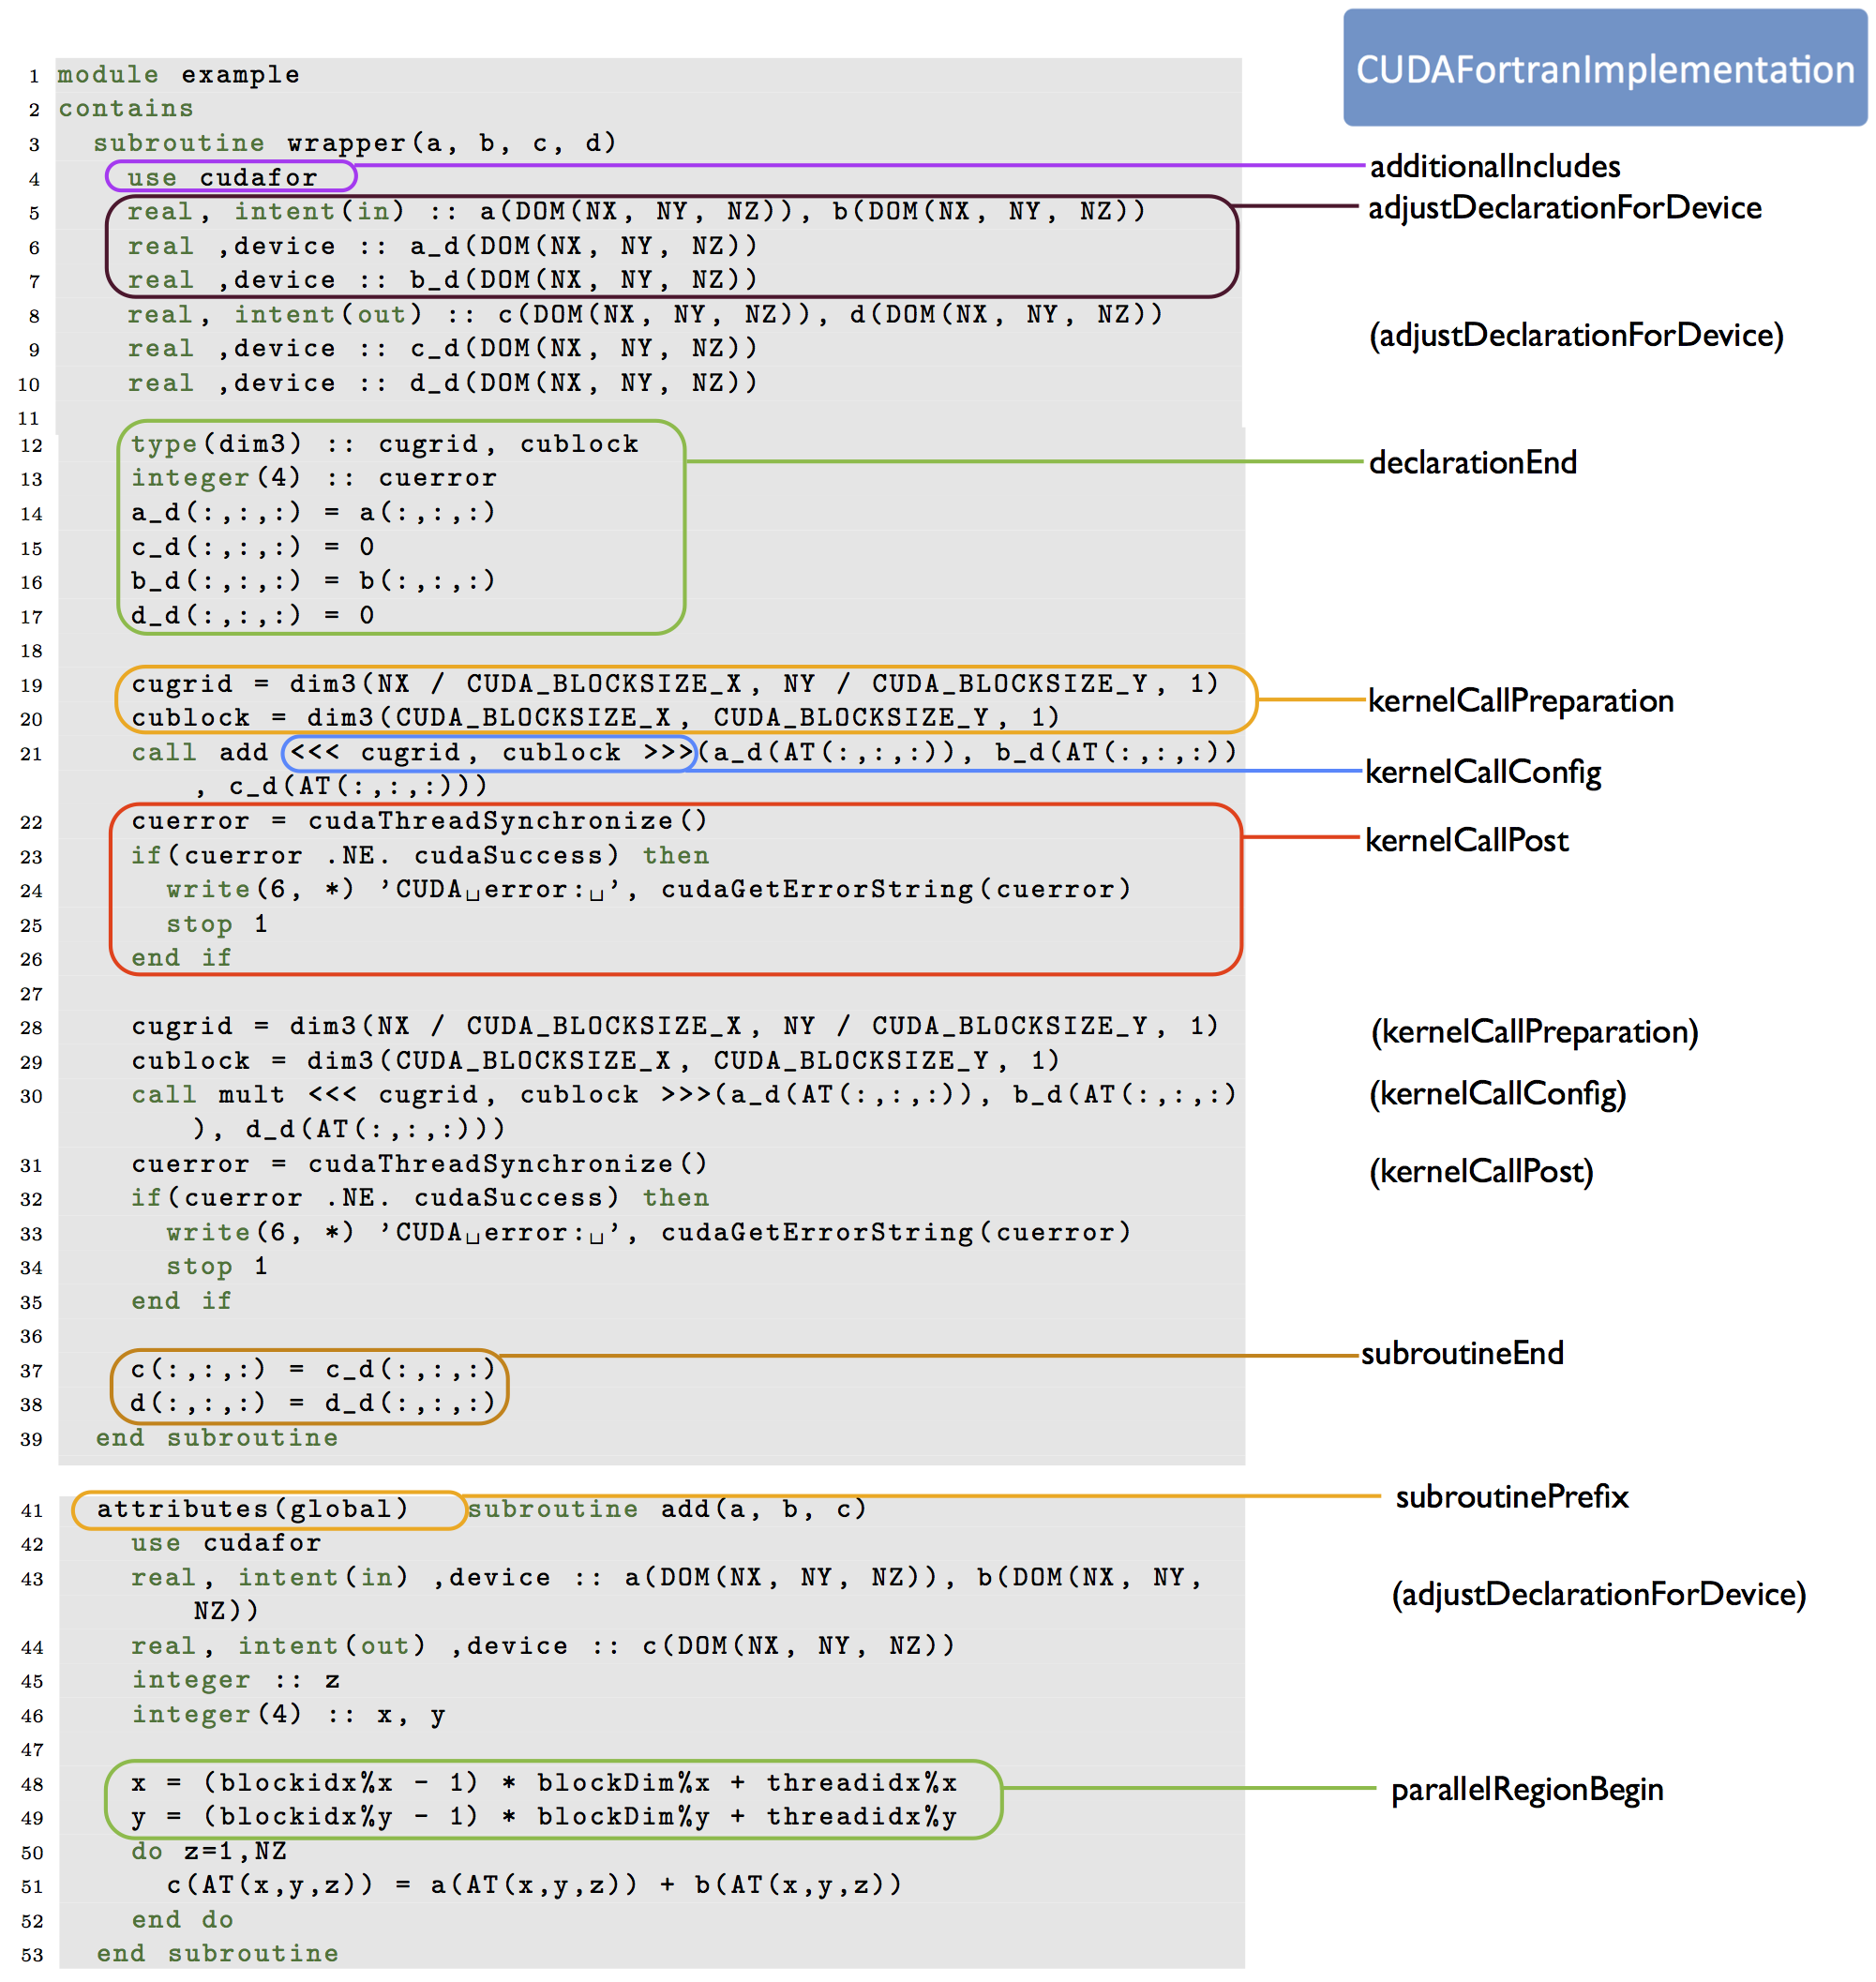
\includegraphics[width=12cm]{figures/implementationMap}
	\caption[Switching Fortran Implementations]{Class member functions of ``FortranImplementation'' classes (Example shown with CUDAFortranImplementation).}
	\label{figure:implementationMap}
\end{figure}
\clearpage

\section{Hybrid Fortran Parser} \label{sub:parser}

In order to interpret the directives introduced in cha~\ref{cha:framework} in the right context, it was necessary to create the parser program outlined in this section. This parser is used by the \verb|annotatedCallGraphFromH90SourceDir| and \linebreak \verb|generateF90fromH90AndAnalyzedCallGraph.py| python scripts (as described in sec.~\ref{sub:pythonScripts}) through subclasses.

This section gives a more detailed view of that parser. Figure \ref{figure:parserStateMachine} shows the state machine pattern that has been used for the parser implementation.

\begin{figure}[htpb]
	\centering
	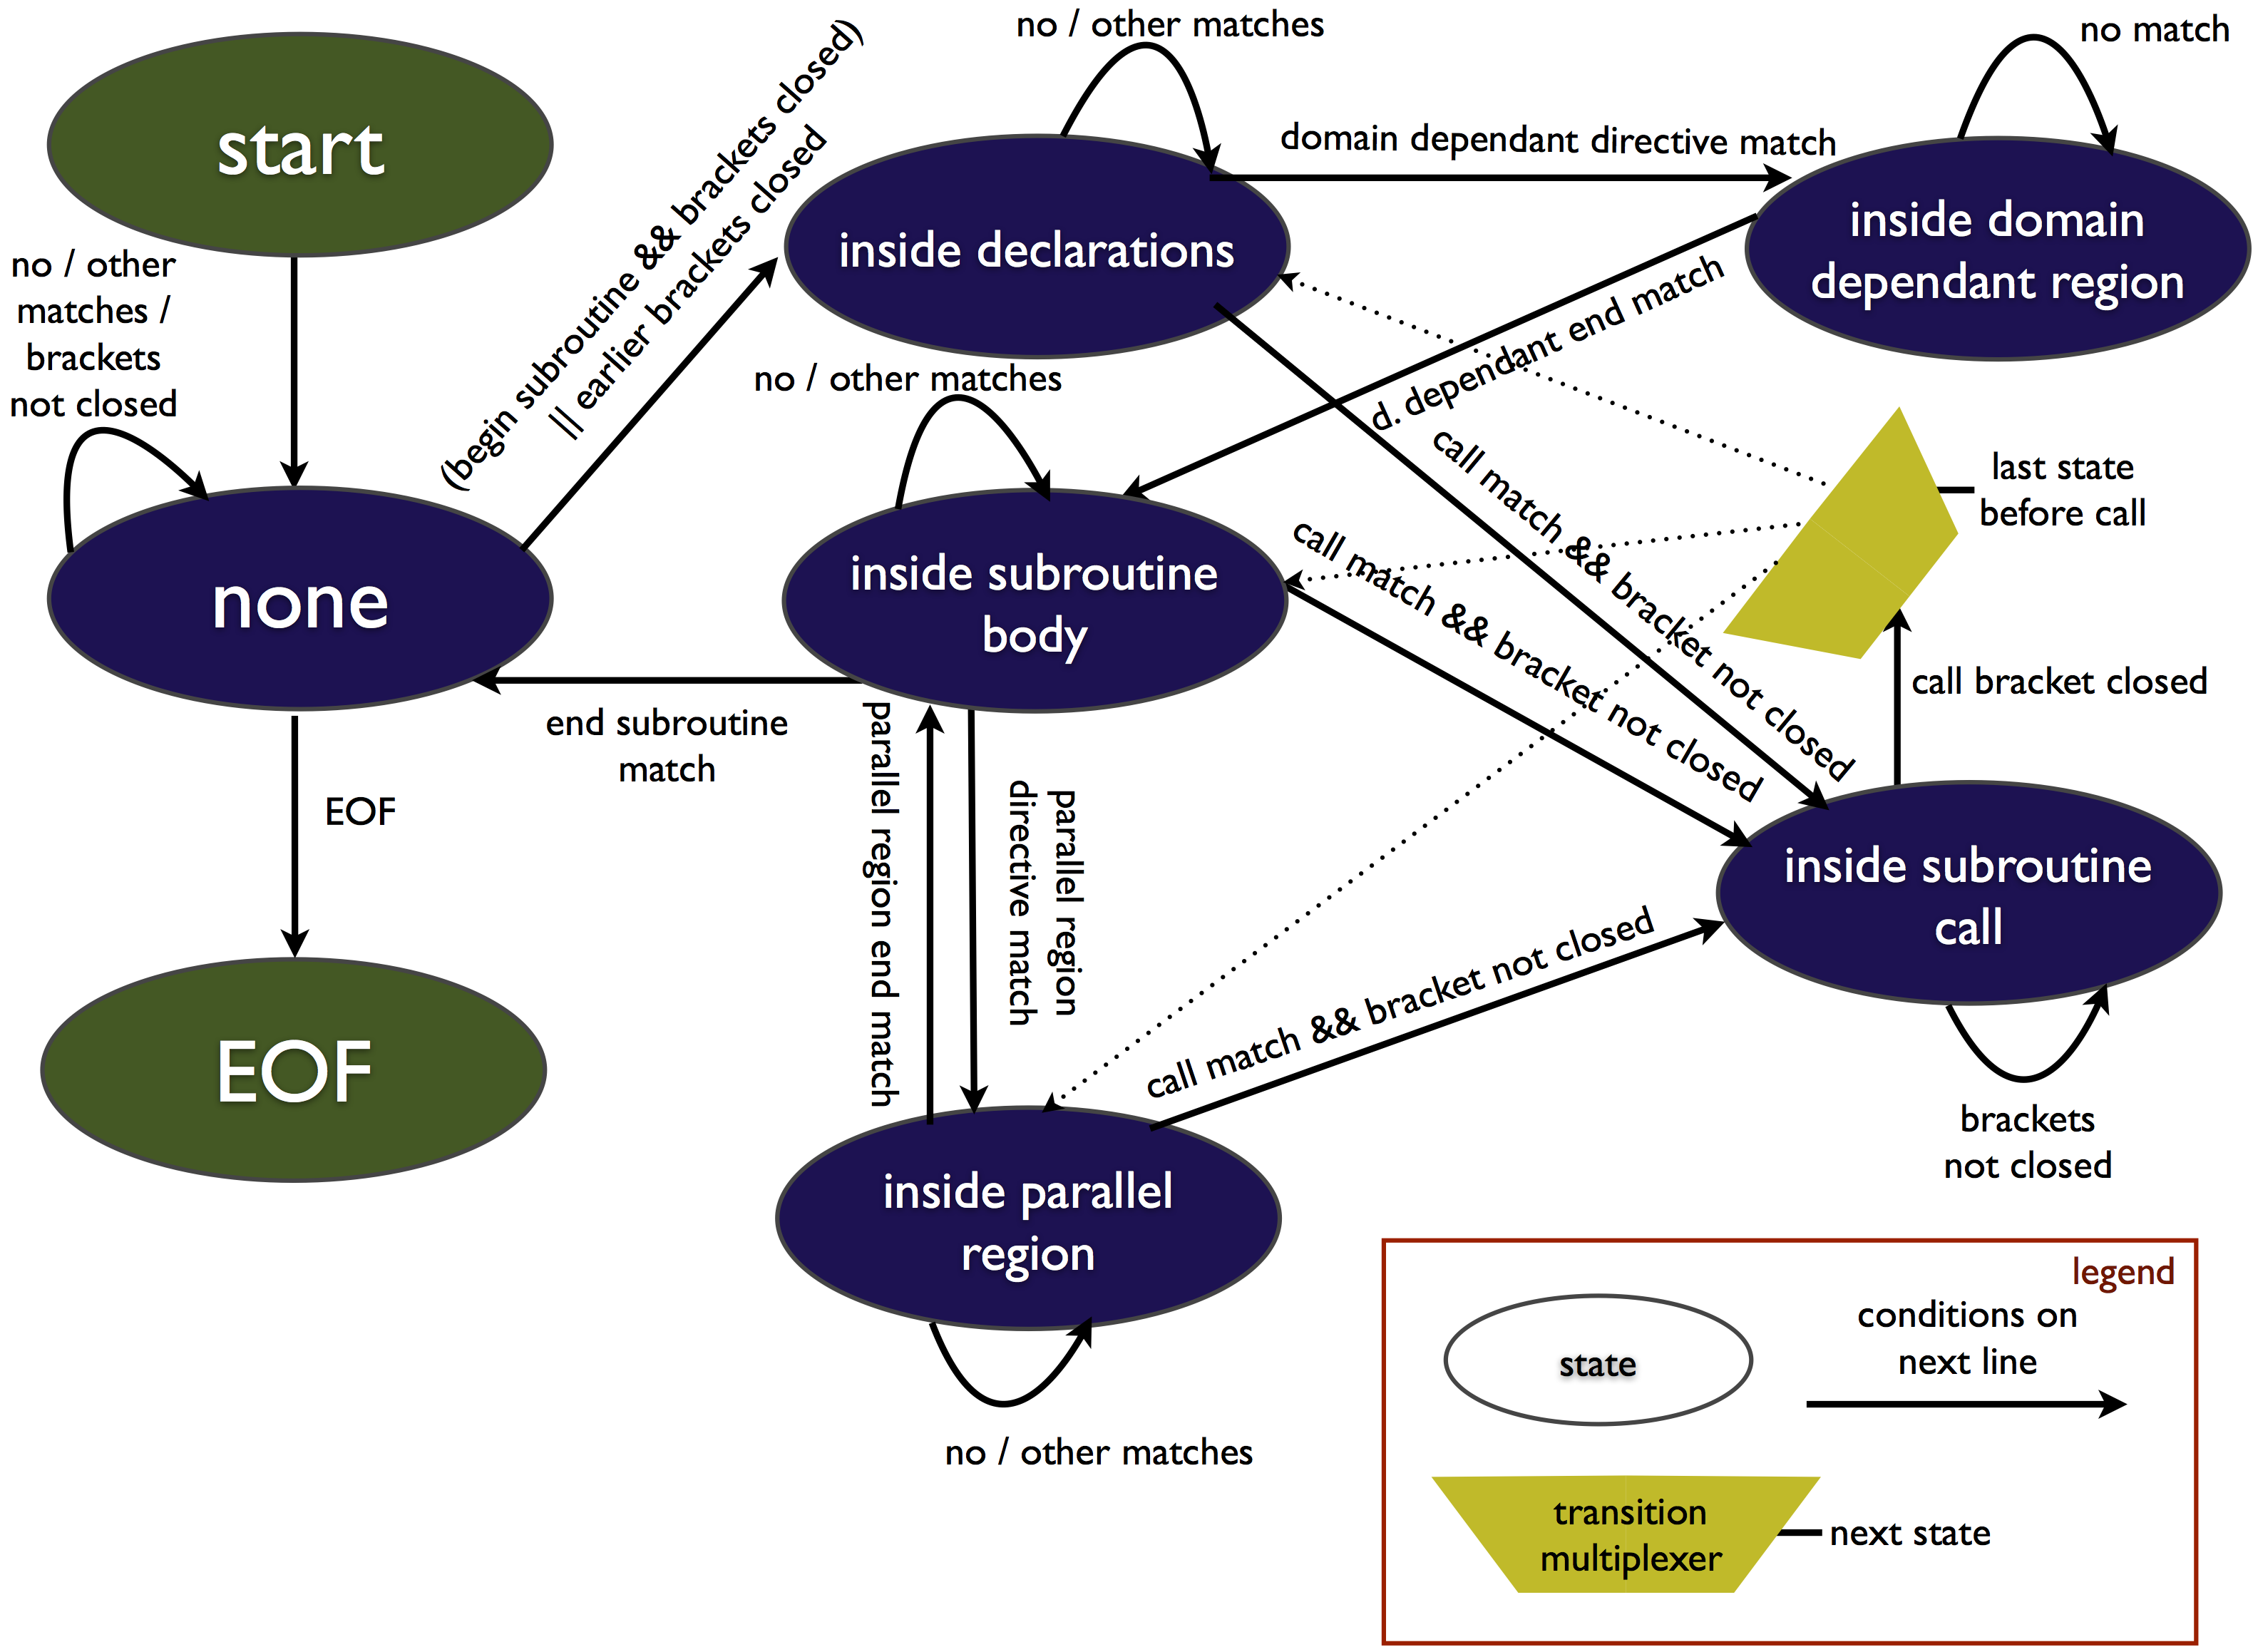
\includegraphics[width=14cm]{figures/parserStateMachine}
	\caption[Parser State Machine]{H90 Parser State Machine.}
	\label{figure:parserStateMachine}
\end{figure}

The state machine design pattern being used here resembles that of a Mealy machine. However, two changes have been applied to the Mealy machine properties:
\begin{enumerate}
  \item The output is being detached from the machine. In other words the \verb|H90Parser| class does not produce any output itself. Its subclasses (as described in sec.~\ref{sub:archHierarchy}) are responsible for that task. This allows large parts of the parser code to be reused for both python programs dealing with h90 source files as described in sec.~\ref{sub:pythonScripts}
  \item A multiplexer is introduced as an additional element in order to reduce the number of states (which matches the way code is being reused in the actual implementation).
\end{enumerate}

% Listing \ref{listing:parserImplementation} gives a simplified overview of how the parser is implemented in code. A few notes:
% \begin{enumerate}
%  \item The matchings are implemented using regular expressions as mentioned in section \ref{sub:archHierarchy}.
%  \item Since python does not have a \verb|switch case| statement, a dictionary has been used instead (functions by state).
%  \item The bracket handling is actually wrapped in its own class (\verb|BracketAnalyzer|) as mentioned in section \ref{sub:archHierarchy}.
% \end{enumerate}
%
%
% \begin{lstlisting}[name=parserImplementation, label=listing:parserImplementation]
%   bracketState = 0
%   state = none
%   stateBeforeCall = none
%
%   function processNoneState(nextLine):
%     if nextLine matches subroutine beginning
%     OR bracketState != 0:
%       /* analyseBracketState will return        */
%       /* the bracket level after nextLine       */
%       /* e.g. if all brackets have been closed, */
%       /* it will return 0                       */
%       bracketState = analyseBracketState(
% 			nextLine, bracketState
% 		     )
%       if bracketState == 0:
% 	processSubroutineMatch(match)
% 	state = inside_declarations
%       return
%
%   function processInsideDeclarationsState(nextLine):
%     if nextLine matches beginning
%     of domain dependant region:
%       processDomainDependantRegionMatch(match)
%       state = inside_domainDependantRegion
%     else if nextLine matches subroutine call:
%       processSubroutineCallMatch(match)
%       bracketState = analyseBracketState(
% 			nextLine, bracketState
% 		     )
%       if bracketState != 0:
% 	stateBeforeCall = state
% 	state = inside_subroutine_call
%
%   function process[...]State(nextLine):
%     ...
%
%   while EOF has not been reached:
%     nextLine = next line from current h90 file
%     choose state:
%       case none:
% 	processNoneState(nextLine)
%       case inside_declarations:
% 	processInsideDeclarationsState(nextLine)
%       case inside_domainDependantRegion:
% 	processInsideDomainDependantRegionState(nextLine)
%       case inside_subroutine_body:
% 	processInsideSubroutineBodyState(nextLine)
%       case inside_parallelRegion
% 	processInsideParallelRegionState(nextLine)
%       case inside_subroutine_call:
% 	processInsideSubroutineCallState(nextLine)
% \end{lstlisting}


% This displays the bibliography for all cited external documents. All references have to be defined in the file references.bib and can then be cited from within this document.
\clear
\bibliographystyle{ieeetr}
\bibliography{references}

% This creates an appendix chapter, comment if not needed.
% \clear
% \appendix

\end{document}